\chapter{Introduction} \label{chapter:intro}

\lettrine{S}{cience} is a theoretical framework that explains the reality of nature. The scientist's vocation is to navigate the huge gap between theory and reality, allowing the understanding of the world where we live.
%
Out of the many science fields at service of human wealth, the most challenging and still far away from being mastered is the comprehension and manipulation of the human body and mind. It is striking how we are finally scratching the understanding of these two entities in the same historical moment, at a point where computers start imitating human reasoning \citep{AlphaGo,googleAIblog,Alom2019} and biological materials are turned into semi-functional organs \citep{Rossi2018}.

The process of understanding is intermingled with the process of creation, as scientific knowledge funded the field of technology. In the past two centuries we witnessed a technology evolution that condensed the collective expertise we accumulated so far into objects belonging, by now, to our daily life.

This boost of technology allowed for the development of novel instruments, and in turn for the accumulation of a broader scientific knowledge. Consequently, the times of all-round scientists left the way to an era in which specialisation is necessary to master and understand a subject, in the hope and trust that piecewise knowledge builds an organic corpus once the effort of many scientists is joined together.

The increasing understanding of how we work - or fail to do so sometimes - together with the discovery of bacteria and the symbiotic or disruptive relationship we have with them, poses novel questions to science: why the body, which is carefully design to function effectively, fails sometimes? And why in these cases it defends itself also against beneficial drugs? But mostly, what can we do to repair such faults?

Our biological and emotional push to change the course of nature to improve our lives lead to the development of ``medical technologies" such as drugs and treatments to aid the body in fighting the agents which attack it. Historically, this proceeded from a process of trial and error of natural substances, to an informed synthesis of artificial drugs to repair the body \citep{Wishart2018}, together with disinfectants \citep{WIDES_database} and antibiotics \citep{ABXdatabaseJhopkins} to fight pathogens: all together, we are closer and closer to the \emph{magic bullet} envisioned a century ago by Nobel Prize Paul Ehrlich, who dreamed of a ``personalised and tailored drug" able to target specific molecular defects while being beneficial to other healthy cells \citep{Strebhardt2008}. A success of the kind will be a life saving technology, and condense in a tiny space centuries of efforts to understand nature.

Given the vast amount of knowledge on the topic, every research task focusses on single, simplified questions to complete the jigsaw. While new problems arise and are answered, new experimental techniques are developed to investigate them. However, the difficulties of studying micrometric systems as cells and bacteria are manifold, as we often do not possess instruments to look at them with the desired level of detail, or without perturbing their natural conditions. Therefore, in the last decades a new investigation approach emerged, proposing to model the systems of interest from the theoretical knowledge gathered so far, in terms of their structure, behaviour and properties.
%
Computational Biology is the field that proposes to do that, implementing those models first and then querying them for properties which are still unknown. At times, this proves to be the only method possible to answer the question posed \citep{Lee2009,Dror2012,Chou2015,Leipzig2016}.

This thesis aims at employing techniques belonging to Computational Biology to answer the specific question of how an artificial molecule behaves within selected biological environments.
%
Thus, while studying a structural biology problem, it places itself at the boundary with the fields of Bioengineering and Medicine: the following introduction is meant to give an overview of the many different challenges these fields have faced in recent years and the solutions found to those challenges, motivating the interest in developing novel molecules as the one which will be described in this work. In particular, two problems are highlighted: the insurgence of drug resistance, and the problem of drug delivery, as they are both addressed by the system in exam. Figure \ref{fig:intro} provides a work flow of this introductory chapter, to help the reader in identifying the sections of interest.

\begin{figure}[p!]
\begin{center}
\Large{\textbf{Motivations of the work: a graphical abstract}}\par\bigskip
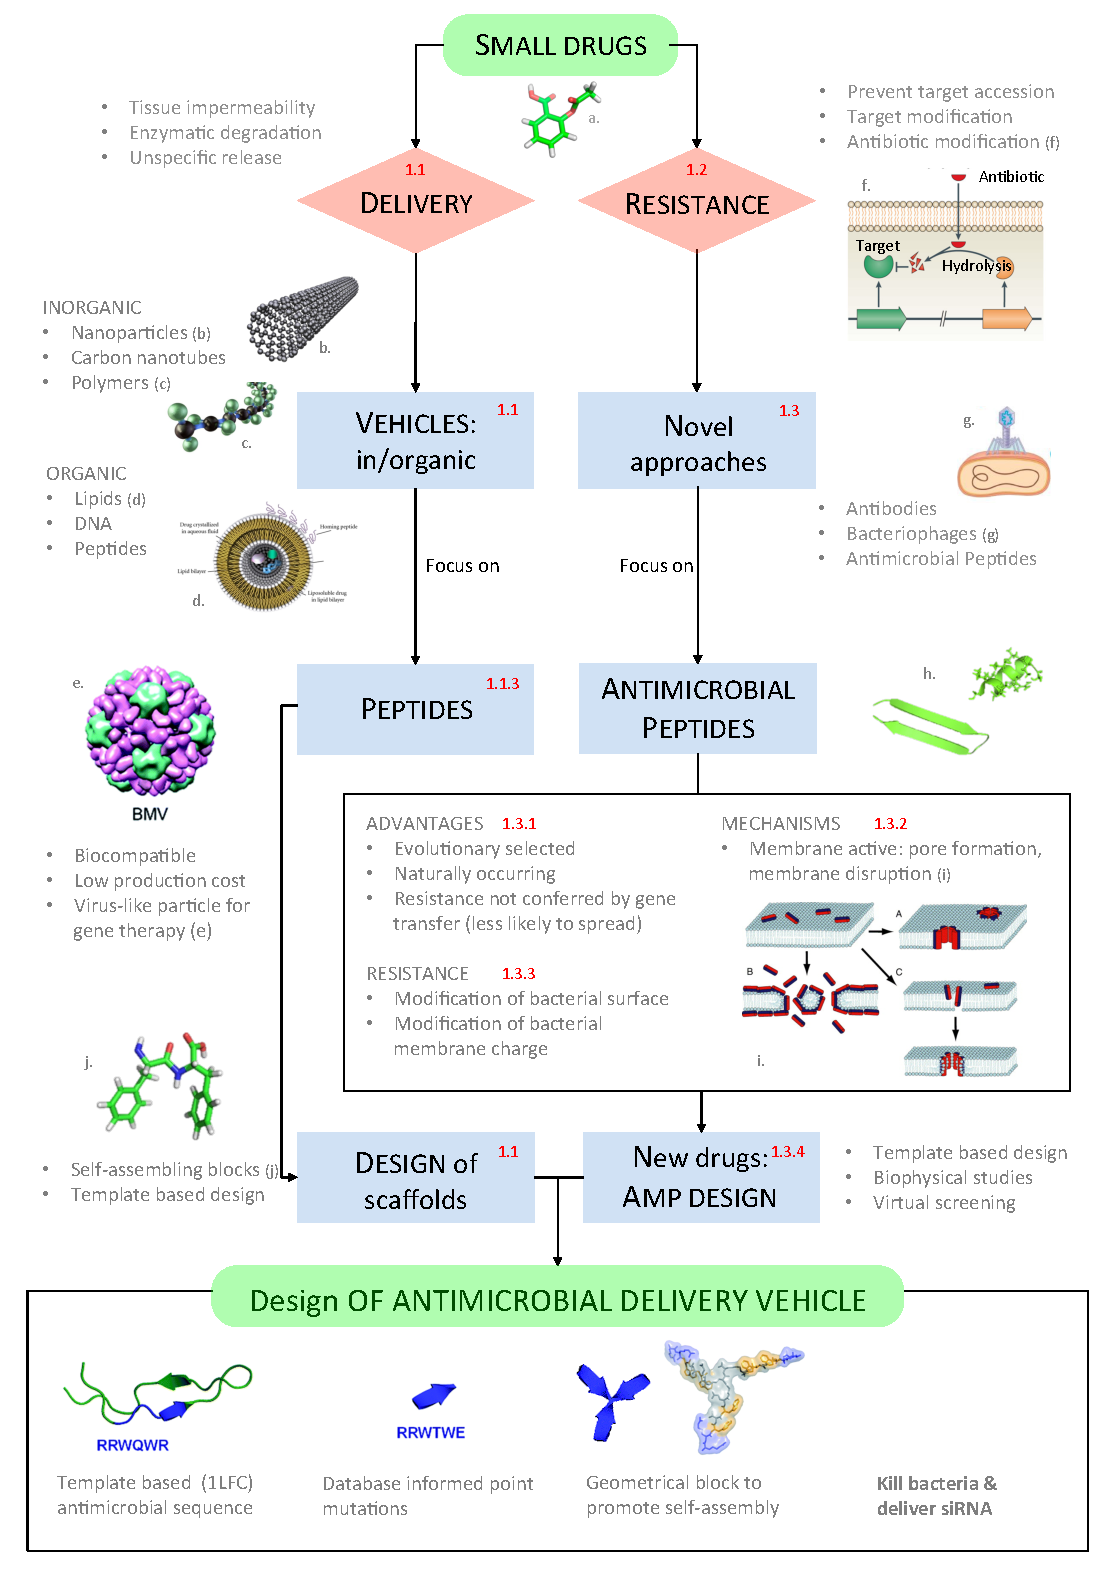
\includegraphics[width = 0.95\textwidth]{1introduction/pics/scheme_intro}
\caption[Graphical abstract of introduction]{Figures a. Acetylsalicylic acid and j. Diphenyl-alanine in bond representation [VMD software \citet{HUMP96}]. Remaining figures adapted from: b. \citet{Blair2014}; c. \citet{phage}; d. \citet{Torres2019}; e.\citet{Nguyen2011}; f. \citet{nanotube}; g. \citet{poly}; h. \citep{lipo}; i. \citet{Schoonen2014}; k. \citet{Castelletto2016}; l. \citet{Kepiro2019}.} \label{fig:intro}
\end{center}
\end{figure}

%\clearpage

\section{Antimicrobial resistance}

For most of the last century, the development of new drugs rotated around the paradigm that a drug is a small inorganic compound (of mass up to 900 Da), which intervenes on a specific target of a mammal or bacterial cell. Very often the targets of interest are (intracellular) proteins: out of the 695 small drugs approved by FDA (the American Food and Drug Administration agency) to target human molecules, 667 acts on proteins. Similarly, 189 of the 198 approved to treat pathogens have a protein as their target
%
(with all the caveats coming from the challenges of identifying an unambiguous target, especially when the drug binds to a protein complex or to a number of closely related gene products \citep{Santos2017}).

In presenting the aforementioned figures, the data were naturally split among the drugs which act on human molecules, ``repairing" a faulty process in the human body, or the ones active against bacteria (commonly named antibiotics) which ``disrupt" the bacterium life cycle in order to kill or prevent the reproduction of the pathogen.
%
It appears evident that the pool of drugs available to the second purpose has a substantially lower number of compounds than the ones addressing human molecules. This comes from the nature of the action they perform: molecules targeting human proteins need to be highly specific to avoid interference with other proteins or with healthy cells, and in a sufficient number to address the variety of diseases affecting the human body.
%
Antibiotic must be non-toxic for human cells as well, i.e.\ their target must not be shared between mammal and bacterial cells, but there is a less stringent requirement on their selectivity against different bacterial species. On the contrary, it is often useful to have a broad-spectrum compound. This cross-species efficacy and at the same time non-toxic property is obtained thanks to the evolutionary relationship among bacterial species, and between bacteria and humans. While the first are closely related, and therefore share homologous proteins with very similar structures, humans have less folds in common with them, allowing for a resilience against bacteria-targeting drugs.
%
To be precise, the set of bacterial species is very diverse and the cross-species effectiveness of some drugs does not extend to the whole bacterial populations. This is actually a positive feature, given the large amount of beneficial bacteria that live in symbiosis with the human body (especially in the gut) and that must be preserved for an optimal wellness.

Nevertheless, in the framework described above, it is understandable that first-time research on antibiotics was satisfied with the development of a handful of potent, broad-spectrum compounds.
%
Penicillin, the first to be synthetically produced, was isolated from a mould in 1928 by Alexander Fleming. It acts inhibiting the formation of a cross-links between particular molecules (peptidoglycan) in the bacterial cell wall, binding to the enzyme responsible for its catalysis, and thus preventing the wall complete formation \citep{Gordon2000} (for further details on the bacterial cell membrane see Section \ref{sec:host-defense-peptides}).
%
As foreseen from Fleming himself in his Nobel Prize acceptance speech, some species of bacteria quickly became immune to penicillin, and this was achieved in many ways: either by production of an enzyme that degrades penicillin, by subtle changes in the structure of the penicillin-binding proteins to prevent such binding, or again by removal of the drug from the cell through specially re-purposed efflux pumps \citep{Lobanovska2017}.

The mechanisms just outlined are not an exceptional characteristic of penicillin, and many drugs lost their effectiveness against some bacteria from their discovery, urging the research of new ones on a constant basis. By now, a broad knowledge has been gathered on how bacteria escape the action of a drug: this understanding helps interpreting the pitfalls of existing drugs and identifying the characteristics sought for new compounds.


\subsection{Mechanisms of antimicrobial resistance to small drugs} \label{sec:AMR_mechs}
Antimicrobial resistance can manifest through many different mechanisms, which can be grouped in three main classes, in line with the three processes mentioned in the example of the penicillin resistant bacteria.

\begin{figure}[h]
\begin{center}
\subbottom[]{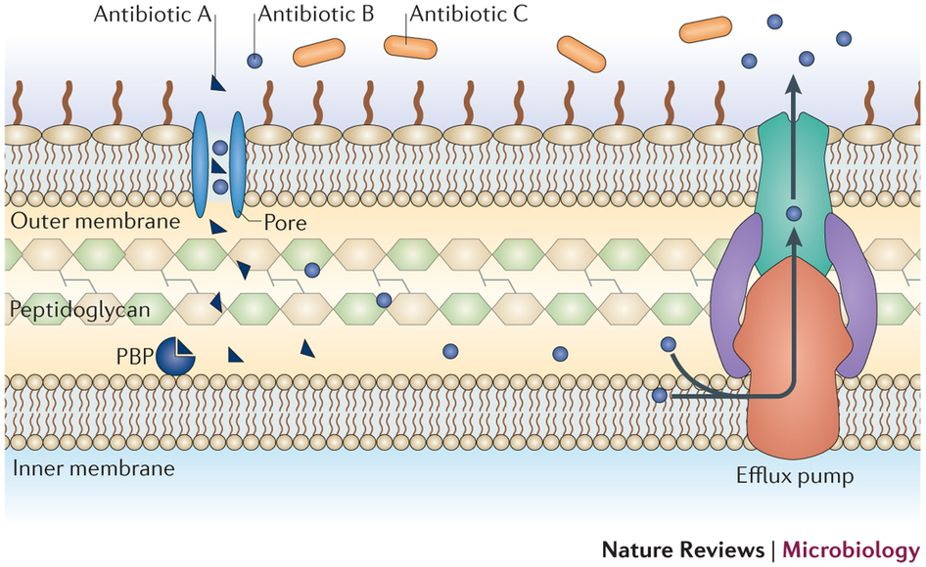
\includegraphics[width=0.6\linewidth]{1introduction/pics/amr1} \label{fig:amr1}} \\
\subbottom[]{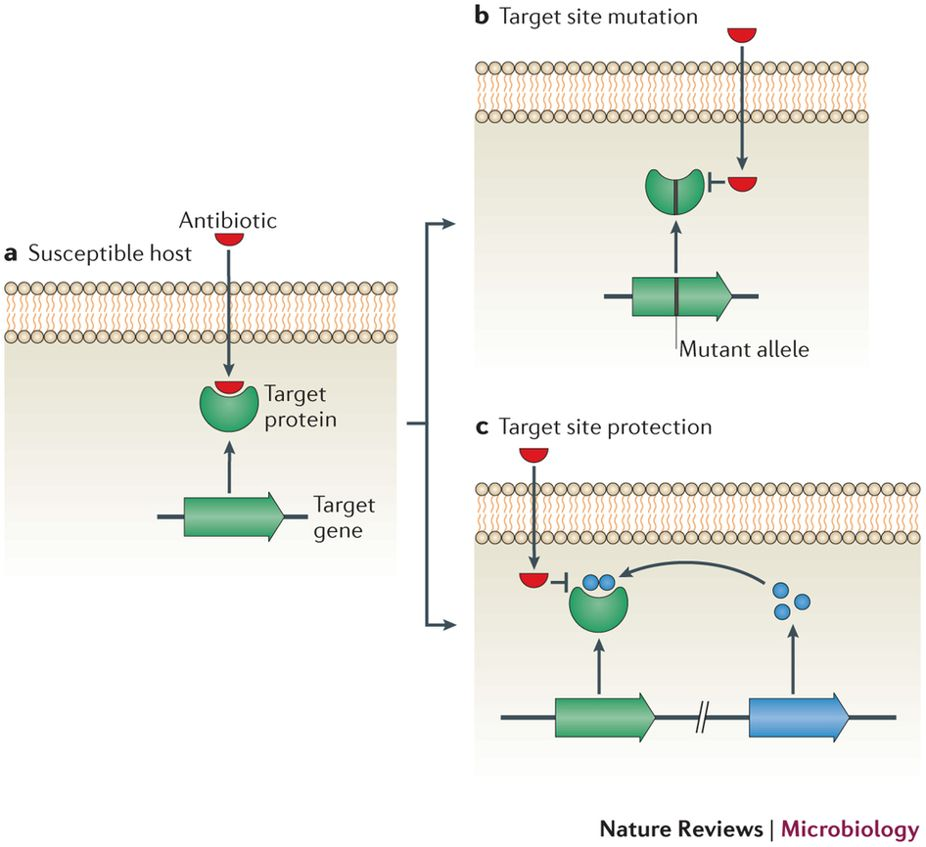
\includegraphics[height = 0.36\textheight]{1introduction/pics/amr3} \label{fig:amr2}}
\hspace{0.5cm}
\subbottom[]{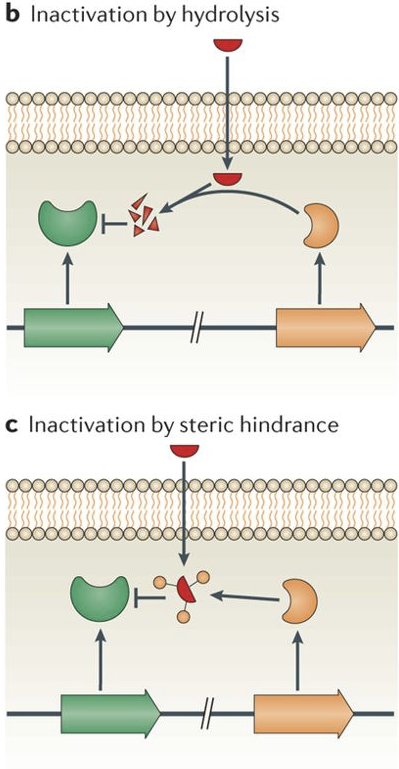
\includegraphics[height = 0.36\textheight]{1introduction/pics/amr4_half} \label{fig:amr3}}
\caption[Mechanisms of antimicrobial resistance to small drugs]{Mechanisms of antimicrobial resistance to small drugs. (a) Removal of antibiotic B by efflux pump and inaccessibility of antibiotic C to the Penicillin Binding Protein target because of membrane impermeability. (b) Target site change via mutation or protection. (c) Direct interactions with antibiotics causing its disruption or structural modification. Reproduced from \citet{Blair2014}.} \label{fig:amr}
\end{center}
\end{figure}

\paragraph{Prevention of access to target}
A first class of resistance mechanisms aims at minimising the intracellular concentration of the antibiotic preventing its penetration or maximising its efflux in the eventuality it has entered the cell (Figure \ref{fig:amr1}).
%
Not all the molecules can enter the cell permeating the membrane, and this holds particularly for hydrophilic antibiotics tackling Gram-negative bacteria, which are intrinsically poorly permeable because of the presence of a double membrane \citep{Delcour2009} (see Section \ref{sec:host-defense-peptides}).
%
These molecules must then be imported into the cell through outer-membrane porin proteins \citep{Vargiu2012,Kojima2013}. Resistance arise when porins are either replaced with more selective channels, which prevent the antibiotic penetration, or down regulated so that the internal concentration of the drug does not reach a critical concentration \citep{Lavigne2013}. Porin-coding genes can also accumulate multiple mutations, to acquire the selectivity they lack in their wild type \citep{Poulou2013}.

A complementary strategy to prevent drug influx is to employ bacterial efflux pumps. Some of them are denominated multidrug resistance (MDR) efflux pumps for their effectiveness in the task and are produced by many bacteria \citep{Floyd2010,Ogawa2012}.
%
Over-expression of such efflux pump is observed in multidrug-resistant bacteria, triggered by exposition to the drug, and proceeding via mutation in the relative regulatory network, \citep{Abouzeed2008}, or simply as a response to environmental signals \citep{Nikaido2011}.
%
Additionally, the genes coding for them can be transferred via plasmids to other bacterial species \citep{Dolejska2013}. Indeed, bacteria are able to exchange genetic material with other individuals via small rings of DNA in a process called conjugation \citep{Sorensen2005}, so that advantageous resistant genotypes can spread quickly across species.


\paragraph{Change or modification of the antibiotic target}
The second class of resistance mechanisms works modifying the antibiotic target: most antibiotics bind to their substrate with high affinity and specificity, thus small modifications in the target structure can disrupt an efficient binding, still allowing the target to maintain its normal function (Figure \ref{fig:amr2}).

Mutations of some residues in the binding pocket (upon mutation in the gene coding for it) or its post-translational protection via addition of chemical groups are equally wide spread strategies.
%
Notable examples of the first include the development of methicillin- (an antibiotic in the penicillin class) resistant strains of S. aureus \citep{Shore2011,Billal2011}. Again, several of these mutations are acquired by horizontal gene transfer from other bacterial species.
%
For the second process, the most relevant mechanism of chemical group addition is methylation, which, for example, is very common when the drug target are rRNA subunits \citep{Long2006}).


\paragraph{Direct modification of antibiotics}
Finally, bacteria can destroy drugs, usually by hydrolysis, or modify them by transfer of a chemical group (Figure \ref{fig:amr3}).
%
The first drug-degrading enzyme discovered was penicillinase \citep{Abraham1988,Lobanovska2017}. Since then, thousands of similar enzymes have been identified that can modify antibiotics of different classes \citep{Livermore2008,Nordmann2011}:
%
these enzymes co-evolves with newly developed drugs, to include in their spectrum of action new compounds of composition similar to the ones they were originally effective on \citep{Woodford2013}.

Antibiotics constituted by large molecules with many exposed hydroxyl and amide groups are instead particularly susceptible to addition of chemical groups. Many enzymes are responsible for this, and according to the chemical moiety added they are grouped in acetyltransferases, phosphotransferases and nucleotidyltransferases \citep{Wright2005}.


%\subsection{Outlook on antimicrobial resistance}
%All together, the recent progress in understanding the mechanisms of antimicrobial resistance has helped in directing the development of new drugs. In particular, it has promoted the modification of existing compounds to escape the resistance developed by bacteria.
%
%It must be noticed that many of the drugs available drugs are bacteriostatic agents as opposed to bactericidal: i.e.\ they prevent the bacterium growth rather than kill it, as they are meant to slow down the damage while host defence mechanisms eradicate them.
%%
%Thus, if an high dosage of a bactericidal agent may extinguish the bacterial population and eradicate the disease, bacteriostatic drugs allow bacteria to start again the reproduction cycle once removed (if the host defence could not properly work), and are thus more prone to ``train" resistant bacteria.
%
%The severity of the AMR treat is such that it has been raised to the status of national emergency in several countries, including UK. Strict regulations on the health, agricultural and food industry sector must be taken to prevent the misuse of antibiotics, as we are leaving the century in which antibiotics were discovered, to enter a phase in which we count the number of the ones loosing efficacy \citep{Oneill2016}.


\section{Alternative antibiotic strategies: antimicrobial peptides}
In the landscape sketched above, the development of novel drugs is of crucial importance. The progress in understanding the mechanisms of antimicrobial resistance has helped this process mainly promoting modification of existing compounds to escape the resistance developed by bacteria.

However, it would be even more beneficial to have at disposal a new paradigm for their design, in order to attack pathogens in a completely novel way, avoiding to target pathways which are known to lead easily to resistance. Several novel materials have been developed for the task, not to rely on small molecules and to exploit different mechanisms of action, for example antibodies, bacteriophages and antimicrobial peptides \citep{Mantravadi2019}.

While the use of pathogen-specific antibodies relies on mechanisms of the host immune system, bacteriophages therapy employs viruses which infect bacteria and archea rather than eukarya.
%
But antimicrobial peptides are the main focus of this thesis: some peptides can have an active role against bacteria, when their sequence possesses specific characteristics, and are thus referred to as antimicrobial peptides. The following subsections will explore their characteristics, modes of action and the response of bacteria against them. It is indeed crucial to understand the knowledge available on these molecules versus the questions that are still open, in order to direct the efforts of future research. This holds in particular when the investigation proceeds by use of simplified models, as the ones employed in Computational Biology. Meaningful results can be obtained only if such modelling is performed in a sensible and informed fashion.

\begin{figure}
\begin{center}
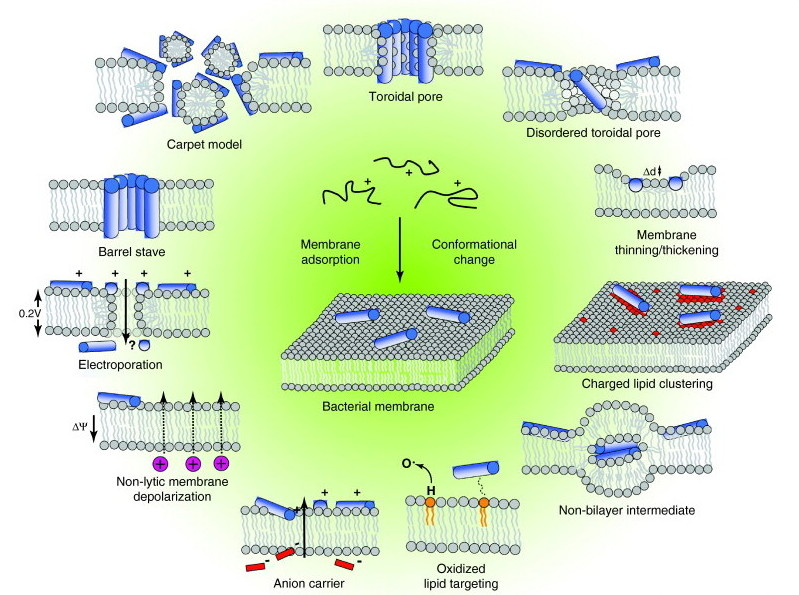
\includegraphics[width = 0.8\textwidth]{1introduction/pics/amp_mech.jpg}
\caption[Modes of action of antimicrobial peptides]{Events occurring at the bacterial cytoplasmic membrane following initial antimicrobial peptide (AMP) adsorption. Reproduced from \citet{Nguyen2011}.} \label{fig:amp}
\end{center}
\end{figure}


\subsection{Membrane active peptides} \label{sec:host-defense-peptides}
Antimicrobial peptides (AMPs) are naturally produced by eukarya, either as stand-alone sequences or embedded in larger proteins, as a first, weak, and broad-spectrum defence against bacteria \citep{Nguyen2011}.
%
This pool of molecules has been selected through evolution to be active against pathogens, suggesting that they will most likely not cause resistance in a near future.

To exploit their potential and engineer AMP-like molecules, a careful characterisation and classification of such peptides must be done. This task has been carried on throughout the past decades, but because of its complexity at present there are many peptides with ascertained antimicrobial activity for which the mode of action is still not fully understood \citep{Ebbensgaard2015}. However, some general characteristics of these sequences and some of the mechanisms they employ have emerged.
%
Unsurprisingly, AMPs are heterogeneous in  sequence, structure, targets and modes of action, to tackle the different challenges bacteria pose. Their size can vary between 6 and 59 amino acids \citep{Brogden2005}: despite being small with respect to the average size of a protein in the human body, these macromolecules are hundreds of times larger than small molecule drugs and as such they penetrate and act on bacteria differently with respect to them.

The most common target of AMPs is the bacterial membrane. Many of them cause disruption of the microbial membrane while others translocate into the cytoplasm to act on intracellular targets, and the combination of the two is not uncommon either \citep{Hancock2006} (Figure \ref{fig:amp}). In general, it is widely accepted that membrane interaction and its relative consequences are a key factor for the antimicrobial activity of AMPs \citep{Nguyen2011}.

As such, we propose a brief overview of the structure of the bacterial membrane \citep{Silhavy2010}, and of its differences with the one of mammalian cells, to better understand how AMPs can be effective and selective on bacteria at once.


\paragraph{Structure of bacterial membrane}
The determinant driving the interaction between AMPs and bacterial membranes is the positive charge that many AMPs present, opposed to the negative charge of the latter \citep{Nguyen2011,Mahlapuu2016}.
%
It is striking that such simple mechanism, based on the presence of a certain number of negatively charged lipids, holds across many bacterial species despite the great variability found in their membrane composition.
%
Indeed, based on the differences in their cell envelope, bacteria are classified into two macro families, Gram-positive and Gram-negative.
%
In Gram-positive bacteria, the cytoplasmic membrane is surrounded by a thick peptidoglycan layer, while for Gram-negative bacteria this membrane (which assumes the name of internal one) is surrounded by a thin peptidoglycan layer and an outer membrane \citep{Silhavy2010,Lin2016} (Figure \ref{fig:membranes}).

\begin{figure}[t!]
\begin{center}
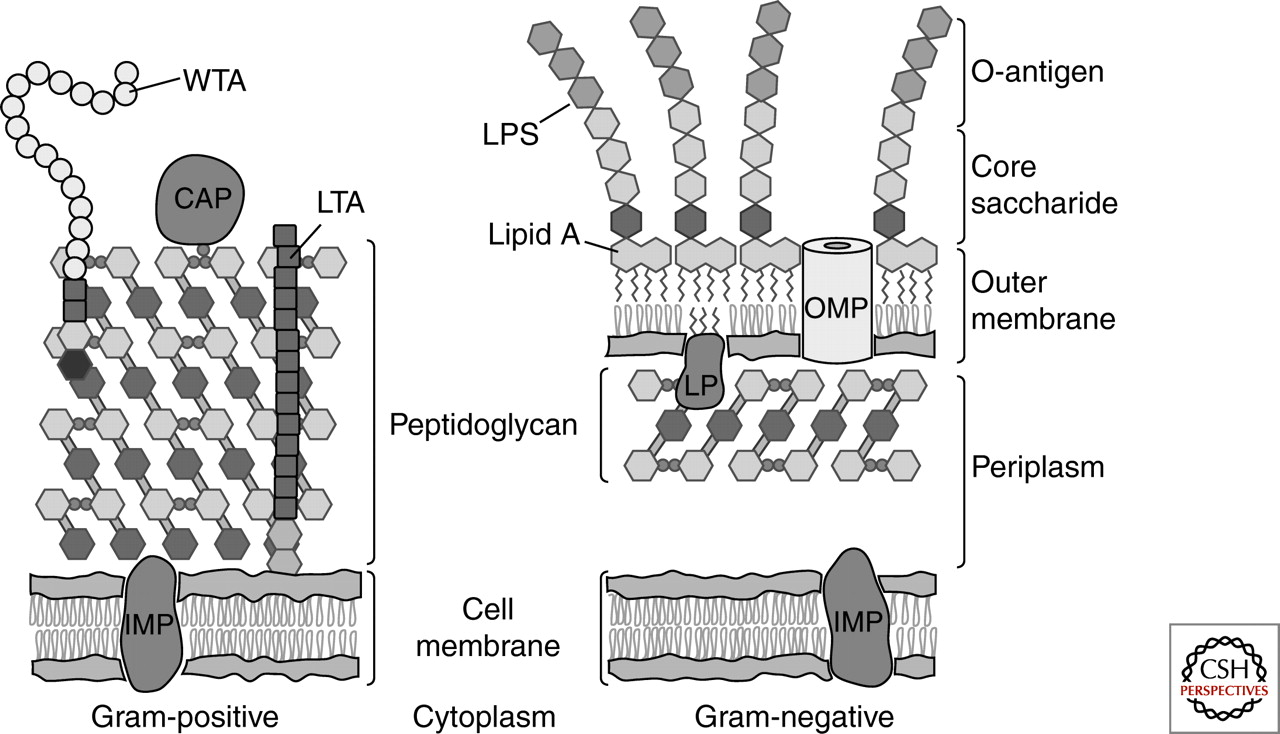
\includegraphics[width = 0.8\textwidth]{1introduction/pics/bacterial_membrane.jpg}
\caption[Structure of Gram-positive and Gram-negative cell envelope.]{Structure of Gram-positive and -negative cell envelope. IMP: integral membrane protein; CAP: covalently attached protein; LTA: lipoteichoic acid; WTA: wall teichoic acid; LP: lipoprotein; OMP: outer membrane protein; LPS: lipopolysaccharide. Reproduced from \citet{Silhavy2010}.} \label{fig:membranes}
\end{center}
\end{figure}

Starting from the inside and proceeding outwards (from bottom to top of Figure \ref{fig:membranes}), the cytoplasmic membranes of both Gram-positive and Gram-negative bacteria are rich in phospholipids like phosphatidylethanolamine, which is neutral, and phosphatidylglycerol, cardiolipin, or phosphatidylserine, which have negatively charged headgroups, highly attractive for positively charged AMPs \citep{Silhavy2010,Lin2016}. This is often sufficient to promote the preferential interaction between this membrane and the peptides - provided they get into its proximity.
%
Perturbation of this membrane is highly disruptive for the bacterium as many functions are associated to it: as bacteria do not possess organelles, all the membrane-related proteins reside and perform their function within the inner membrane.

In the case of Gram-negative bacteria (Figure \ref{fig:membranes}, right), the inner membrane, together with the outer one, delimits the periplasm space, an aqueous cellular compartment, which allows the sequestration of harmful substances and the transport of nutrients.
%
Inside the periplasm is situated the peptidoglycan cell wall. This substance is made of a disaccharide cross-linked by penta-peptide side chains, and these repeated units constitute the rigid skeleton of Gram-negative cells \citep{Gan2008}. Peptidoglycan is fundamental for cell life as its damage results usually in living but not viable cells \citep{Joseleau-Petit2007}.

the outer membrane is grafted to the cell wall through Braun’s lipoproteins (or LPP) \citep{Asmar2018}. This membrane presents an asymmetric structure: phospholipids are present in the inner leaflet, while the outer one is composed of glycolipids, mainly lipopolysaccharides (LPS) \citep{Silhavy2010}. These complex molecules consist of lipid A, which presents multiple fatty acids, and a polysaccharide \citep{Raetz2002}. The polysaccharide is made of an inner core, covalently bond to the lipid, an outer core, and finally a repetitive glycan polymer (O-antigen). The O-antigen (top right in Figure \ref{fig:membranes}) is the molecule exposed by Gram-negative bacteria to the external environment and thus is the target of antibodies recognition.

Given the complexity of the Gram-negative cell envelope, and especially the presence of the LPS layer, these bacteria are particularly impermeable to hydrophilic molecules, which are usually imported within the cell through porins and similar transmembrane proteins.

For Gram-positive bacteria (Figure \ref{fig:membranes}, left) the inner membrane is enveloped in a thick peptidoglycan layer. If its thickness in Gram-negative bacteria reaches a few nanometers, in Gram-positive ones it spans from 30 to 100 nm. This thick layer is threaded by long anionic polymers (the teichoic acids), mainly composed by glycerol phosphate, glucosyl phosphate, or ribitol phosphate repeats \citep{Swoboda2009}. Disseminated in this layer there are several surface proteins with various functions, among which adhesins, which attach to components of the host extracellular matrix.

Gram-positive membranes are generally more permeable because they do not possess a double-membrane structure, nevertheless the peptidoglycan layer they are coated with constitutes a challenge for drug delivery.


\paragraph{Comparison with mammalian membrane}
The fact that AMPs tackle negatively charged membranes is crucial for their selectivity, i.e.\ that they are harmless for the mammalian cells they are produced from \citep{Glukhov2005}. This is possible because mammalian cells have a different membrane composition. They present a single membrane, which is rich in proteins (up to 50\% of its volume) and in lipids, and a small percentage of carbohydrates, mainly embedded in glycoproteins, which promote cell-cell recognition.

The lipidic component is abundant in zwitterionic phospholipids such as phosphatidylethanolamine, phosphatidylcholine, and sphingomyelin, providing a neutral net charge. \citep{Spector1985,vanMeer2008}.
%
Furthermore, the mammalian cell membrane has a high content of cholesterol \citep{Yeaman2003, Lai2009}, a sterol fat, which is proposed to stabilise the membrane regulating its fluidity across different physiological temperatures, and is also though to favour a better accommodation of the perturbations caused by AMPs \citep{Zasloff2002}.
%
Strictly speaking, some negatively charged lipids are present in a few mammal cell types, however they are located in the inner leaflet, while the zwitterionic phospholipids are more abundant in the outer leaflet, in an asymmetric composition \citep{vanMeer2008,Matsuzaki2009}.
%
This structure promotes weaker interactions between AMPs and mammalian cells with respect to bacterial ones, as the former is driven mainly by hydrophobic interactions, while the latter by electrostatic ones.

Another relevant difference between bacterial and mammalian cells is that the first ones have typically a higher transmembrane potential - the difference of electrostatic potential between the inside and the outside environment. For bacteria it falls between $-130$ and $-150$ mV, while for mammalian cells between $-90$ and $-110$ mV \citep{Yeaman2003,Matsuzaki2009,Ebenhan2014}.
%
Given that a potential generates an electric field across the membrane, the higher this is, the higher the resulting electric field pointing from outside to inside the cell. A field in such direction pushes cationic compounds on the outside of the membrane toward the membrane itself. Therefore a stronger bacterial transmembrane potential may promote an enhanced - and thus disruptive - interaction of AMPs with the cell, contributing to AMPs selectivity between bacteria versus mammals \citep{Yeaman2003}.


\subsection{Common mechanisms of action of AMPs} \label{AMP_mechs}
Investigating the perturbation and disruption of a bacterial membrane by antimicrobial peptides is a key point of this work, therefore it is important to highlight the mechanisms known so far through which AMPs reach this outcome.
%
As already mentioned, many AMPs have a positive charge which facilitates the binding to the membrane via charge-charge recognition; accordingly, Arginine and Lysine residues are usually abundant in AMPs sequences. However, the disruptive action takes place through the interaction of AMPs with the hydrophobic core of the membrane, therefore their sequences contain also hydrophobic aromatic residues, especially Tryptophan, which favours the anchoring to the lipid core \citep{Chan2006}.
%
Overall, AMPs resort often to adopt an amphiphatic structure to segregate the hydrophilic from the hydrophobic amino acids and thus to act at the interface between membrane and solution. It is interesting to notice that some of them fold into the active structure only nearby the membrane, as they can expose their hydrophobic components to face its core, while in solution these ones are preferentially buried inside the peptide fold to be screened from the solvent \citep{Nguyen2011}.
%
Common folds adopted by AMPs are both $\alpha$-helix or $\beta$-sheet rich structures. Amphiphatic $\alpha$-helices present a charged side which is tailored to face towards the phospholipid head groups and an hydrophobic ones which is favourably buried into the acyl chains core.
%
A similar arrangement is found for structures rich in $\beta$-sheets, such as $\beta$-hairpins (Figure \ref{fig:amp_structure}).


\begin{figure}[t!]
\begin{center}
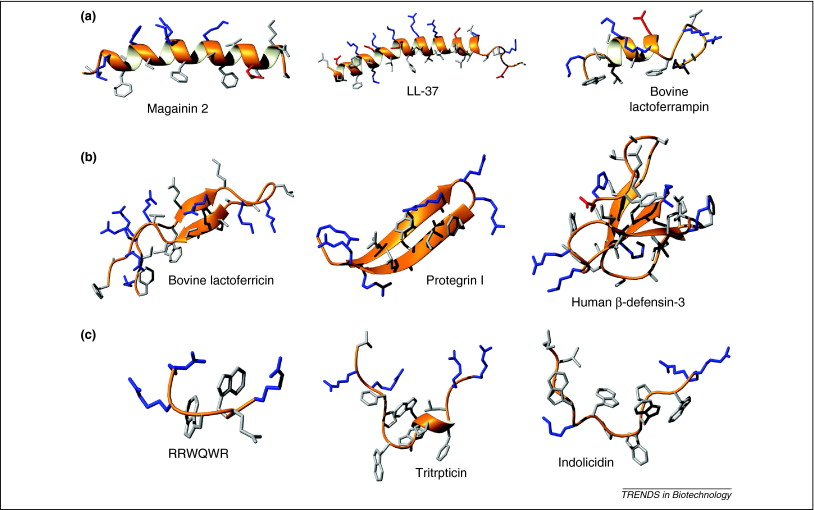
\includegraphics[width = 0.8\textwidth]{1introduction/pics/AMP_many.jpg}
\caption[Structure of some known AMPs.]{Structure of some known AMPs. (a) Helical structures, (b) $\beta$-sheet structures, (c) disordered ones. Reproduced from \citep{Nguyen2011}.} \label{fig:amp_structure}
\end{center}
\end{figure}


\paragraph{Membrane disruption} Several models have been proposed to describe the exact mechanisms of AMPs penetration after they bind to the cytoplasmatic membrane, and how their combined action leads to membrane permeabilization (Figure \ref{fig:amp}) \citep{Brogden2005,Nguyen2011}.

For a single copy of an amphiphatic helical AMP, the proposed mechanism of action suggests that initially the peptide is attracted with its charged side to the membrane and lies parallel to its plane, with the hydrophobic side unfavourably exposed in solution. Then the helix rearranges to have the two faces in the respective favourable regions. Subsequently, the helix axis starts to form an angle with the membrane plane, and finally inserts deeper into the lipid core, often spanning the full membrane thickness \citep{Ebenhan2014}.
%
Similarly, for $\beta$-sheet rich structures, it is suggested that they insert within the membrane after a first flat approach.
%
The final insertion arrangement depends on the peptide characteristics and length, the presence of kinks in its structure (in case of helices), and the interactions with other copies of the peptide.

The picture becomes more complex for oligomer-mediated insertion, i.e.\ when the action is triggered by the combined action of many copies of the peptide.
%
At low peptide to lipid ratio, the favourable configuration is represented by peptides lying parallel to the membrane plane as described previously \citep{Yang2001}. An increase in peptide concentration triggers the transition to an inserted state: the organisation of AMPs inside the membrane core can assume different configurations, as described below \citep{Brogden2005,Nguyen2011,Ebenhan2014,Mahlapuu2016} (see Figure \ref{fig:amp}).

The ``barrel-stave" model proposes that AMPs insert perpendicularly into the bilayer.
Recruitment of peptides in the same area results in the formation of a transmembrane pore with a central lumen. The walls of the pore are constituted by the hydrophilic face of the peptides, while their hydrophobic side is interacting with the lipid tails around the pore. This model is adopted, for example, by the $\alpha$-helical AMP alamethicin, which forms voltage-dependent ion channels by aggregation of four to six molecules \citep{Spaar2004}.

In the ``toroidal" pore model instead, the insertion of peptides forces the phospholipid to bend continuously from one leaflet to the other.
%
The toroidal model differs from the barrel-stave model as the peptides are always associated with the lipid head groups even when they are perpendicularly inserted in the lipid  bilayer. Toroidal pores are induced by $\alpha$-helical magainins, protegrins and melittin \citep{Yang2001,Matsuzaki1996,Hallock2003}, and lead to membrane perturbation which extends further away from the pore than in the barrel-stave case. As a comparison, alamethicin induced barrel-stave pores have an inner and outer diameters of 1.8 nm and 4.0 nm respectively \citep{Spaar2004}, while magainin-induced toroidal pores have variable sizes, with an inner diameter of 3.0-5.0 nm and an outer diameter of 7.0-8.4 nm \citep{Matsuzaki1997}.

Finally, in the ``carpet" model, the accumulation of AMPs on the surface of the membrane, laying parallel to it, causes tension in the bilayer: the membrane is disrupted by them in a detergent-like manner, leading to the formation of micelles.
%
The critical threshold concentration triggers a cascade effect, as the first disruption allows the penetration of AMPs in the inner side of the bilayer. The cooperation between peptides on both sides of the lipid membrane enhances the AMP-induced curvature causing accelerated disruption.
%
The ``carpet" model mechanism is observed for peptides presenting an $\alpha$-helical structure (like melittin \citep{Ladokhin2001}) or for several helices connected by short loops (ovispirin \citep{Yamaguchi2001}).

The prevalence of examples with an helical structure derives from the fact that the understanding of how helical AMPs function is often easier than the one of $\beta$-sheet rich structures.
%
Indeed, helices have a well defined fold (at least nearby the membrane environment), a compact structure, and often a clear segregation of complementary patches that can attract other copies of the peptide and thus promote the self-assembly process necessary for pore formation.

On the contrary, many $\beta$-sheet AMPs have a more flexible structure, and more diversified mechanisms of action \citep{Nguyen2011,Mahlapuu2016}.
%
AMPs rich in $\beta$-sheets can be divided into $\beta$-hairpins and peptides from the defensin family \citep{Nguyen2011}.
%
Many representative of the first class disrupt bacterial membranes via formation of toroidal pores: as an example, porcine peptide protegrin I assembles into a $\beta$-barrel structure when in contact with anionic membranes and triggers toroidal pore formation. Instead, it folds into $\beta$-sheet aggregates on the surface of cholesterol containing membranes, thus acting selectivity on bacterial membranes only \citep{Tang2009}.

In the case of defensins, many mechanisms are known according to the specific member of the family \citep{Lehrer2004,Kagan1990,Takeuchi2004}.
%
Although various descriptions of membrane damage have been reported, and include ion channels, transmembrane pores and extended rupture of the membrane, they are likely related, being a modulation of a similar acting principle.


\paragraph{Alternative mechanisms of action} Finally, many non-lytic mechanisms are suggested for AMPs, especially for $\beta$-sheet structures: defensin A from P. terramovae reduces the cytoplasmic potassium concentration \citep{Brogden2005}, partially depolarising the inner membrane. Tachyplesin from horseshoe crabs is able to bind to the minor groove of DNA, interfering DNA–protein interactions \citep{Yonezawa1992}.
%
Bovine lactoferricin can act synergistically with other antimicrobial agents by affecting the transmembrane potential and proton-motive force, resulting in inhibition of ATP-dependent multi-drug efflux pumps \citep{Gifford2005}.
%
Moreover, after translocation within the cell, bovine lactoferricin can also inhibit DNA, RNA and protein synthesis.

Section \ref{sec:capzip} will treat in detail the functioning of this AMP, distinguishing its role as membrane active peptide as opposed to intra-cellular targeting compound. Indeed, many works have focussed on locating the section of the sequence performing the membrane disruptive activity \citep{Tomita1994,Schibli1999}, to understand whether it retains the efficacy regardless of the fold.
%
These type of investigations provides the discovery of minimal functioning antimicrobial blocks, which promotes the understanding of how AMPs work in general, and boost the design of synthetic AMPs tailored for specific functions.


\subsection{Mechanisms of resistance to AMPs}

Antimicrobial peptides were introduced here as a class of new drugs and a possible solution to the crisis of antimicrobial resistance. Any new drug entering the pool of the clinically approved compounds is (at least temporary) a solution to the problem of resistance; but it must be clarified that bacteria can develop resistance to AMPs too.
%
Nevertheless, this is generally not based on dedicated genes that are conferred by horizontal gene transfer, as in the case of many antibiotics resistance mechanisms \citep{Peschel2006}. Because of that, a certain increase in bacterial resilience after exposure to the peptidic drug is to be expected, but it is less likely to spread quickly to other species.

Some of the mechanisms of AMPs resistance are similar to the ones employed by bacteria to counteract small molecule drugs, for example over-expression of efflux pumps to dispose of AMPs, degradation of the peptide by extracellular enzymes and sequestration by the bacterial or biofilm matrix to prevent accession to the target \citep{Peschel2006}.

Differently with respect to antibiotics hydrolysis, AMPs proteolitic degradation is operated by proteases, secreted on the extracellular side of the membrane specifically to destroy other proteins. Linear AMP are more prone to this type of degradation \citep{Sieprawska-Lupa2004}, as opposed to the ones presenting disulfide bonds \citep{Peschel2006}, such as defensins, which nevertheless can be hydrolysed by more specific enzymes \citep{Nelson2011}.

But the most specific mechanism of AMPs resistance concerns modifications of the bacterial cell envelope: bacteria modify the characteristics of their surface to prevent the efficient binding of an AMP, even in the eventuality that the peptide reaches the bacterial envelope intact. 
%
The target of such modifications are different for Gram-positive and Gram-negative bacteria, according to their distinct cell envelopes.
%
for example, Gram-positive bacteria change the structure of their teichoic acids (TA): D-Alanylation of TA observed in S. Aureus adds a positive charge to it, reducing the attraction of cationic AMPs and in turn increasing the cell wall density, so reducing the surface permeability \citep{Saar-Dover2012}.

In Gram-negative bacteria a positive charge can be added to lipopolysaccharides (LPS) by addition of amine-containing molecules \citep{Moskowitz2004} or by removing phosphate lipids (which have a negative charge) from lipid A \citep{Wang2006lpx}.
%
Moreover, the cytoplasmic membrane can be modified as well, as this is the final target of many antimicrobial peptides: in the eventuality that AMPs successfully reach this membrane, they are attracted to its surface by the negative charge of the lipids composing it, in particular phosphatidylglycerol (PG) and diphosphatidylglycerol (DPG, also called cardiolipin). Their negative charge can be masked by amino-acylation of the PG head group, so that the final compound repels AMPs through electrostatic interaction \citep{Peschel2001}; alternatively the overall rigidity of the cytoplasmic membrane can be enhanced, by an increase in saturated acyl chains which has been proven to confer resistance \citep{Kumariya2015}.
%
To be noticed that resistant bacteria often employ many of the aforementioned strategies at the same time \citep{Band2014}.


\subsection{Principles of AMP design} \label{sec:amp_design}

The study and classification of AMPs provide knowledge on the characteristics a sequence must have to perform an antimicrobial function.
%
As discussed in Section \ref{AMP_mechs}, there are some features which, comprehensively, help in discriminating AMPs against non antimicrobial peptides. The constantly increasing amount of data available is gathered in several curated databases \citep{APD3,DBAASP2,dbAMP,antiBP2,amPEP}, which catalogue AMPs (or subclasses of them, like membrane active, biofilm active or haemolytic peptides) based on such features.

To recapitulate, AMPs are charged moieties, usually cationic, and their potency, but also their haemolytic activity, is often related to their net charge \citep{Jiang2011}. They can assume both $\alpha$-helical and $\beta$-sheet fold; which helps creating an amphiphatic structure, to accommodate both the charged residues mentioned and the hydrophobic ones they possess as well. Finally, they need good solubility to prevent aggregation in the aqueous environment before reaching the target.

%We recapitulate below a few key characteristics which are peculiar of AMPs. To be noticed that while some are easily retrievable from the sequence of the peptide, others imply direct experimental measures to be retrieved:
%\begin{itemize}
%\item \textbf{Structure}: both $\alpha$-helical and $\beta$-sheet rich AMPs exist, as well as mixed structures. Short helices ($\sim$ 22 amino acids) and short $\beta$-sheets ($\sim$ 10 amino acids) are particularly common. When screening a potential AMPs, it must be considered that the fold adopted by the peptide close to the membrane environment might be different with respect to the one in solution.
%%
%\item \textbf{Charge}: AMPs are charged moieties, usually cationic (up to $\sim + 10\,e$), with fewer anionic examples (like dermcidin). Among cationic ones, not all the positive amino acids have equal role, for example Arginines are more effective than Lysins \citep{Chan2006}. The potency, but also their haemolytic activity, are often directly related to the amount of charge \citep{Jiang2011}.
%%
%\item \textbf{Hydrophobicity}: AMPs contain also hydrophobic residues, usually with abundance of aromatic chains and specifically Tryptophan \citep{Chan2006}, as they must insert and anchor into the lipid core of membranes, which is an hydrophobic environment.
%%
%\item \textbf{Amphipathicity}: to host both the charged and hydrophobic residues, most AMPs organise themselves in an amphiphatic structure, i.e. the two types of amino acids side chains are located on the opposite sides of the peptide.
%%
%\item \textbf{Solubility}: AMPs need good solubility to prevent aggregation in the aqueous environment they float in before arriving to the membrane. Aggregation would most likely impede their optimal interaction with the membrane.
%\end{itemize}

The knowledge of AMPs sequence-activity and structure-activity relationships is beneficial to design new peptides with improved characteristics. In particular, improved specificity against bacterial species; stability against the action of proteases (allowing a longer residence time in the body); and low cytotoxicity at the therapeutic dose required.
%\begin{itemize}
%\item \textbf{specificity} against particular bacterial species;
%\item \textbf{stability} against the action of proteases, thus allowing a longer residence time in the body;
%\item \textbf{low cytotoxicity} at the therapeutic dose required (so an high therapeutic index).
%\end{itemize}
The need for such improved peptides lies in the fact that natural AMPs constitute a first broad spectrum defence that our body employs against infectious bacteria, and thus they are often of mild potency. However, foreseeing their application as future drugs, it is desirable to tailor them to fulfil different criteria according to the infection to treat.
%
At the present state of the art, a golden rule for the design of such sequences is still missing, however several methodological approaches to AMP design have been explored, and they can be grouped in three main lines: template based studies, biophysical studies and virtual screenings \citep{Fjell2011}.

\paragraph{Template based studies}
The main idea behind template based methods consists in modifying existing antimicrobial sequences in the direction of the desired characteristics.
As such, the effort is restricted on a subset of all possible sequences.
%
The most widely explored templates are helical peptides, for their short sequences and because several of them (cecropin, magainin and protegrin) have been well characterised \citep{Wang2015}.

Alanine scanning \citep{Migon2018} and all amino acids scanning \citep{Hilpert2005} performed for every residue in a sequence provide information on the role of each of them, pointing at the most suitable mutations. High-throughput methods for synthesis and characterisation allow nowadays for such thorough investigation in the case of short AMPs \citep{Hilpert2005}.
%
%Alternatively, simpler approaches aim at designing peptides with enhanced charge and amphiphilicity, as these characteristics are deemed crucial for their effectiveness (see the paragraph above) \citep{Wang2015}.

However, these methods focus on single amino acids and can not take into account the interplay between residues, nor the three dimensional structure of the peptide. Because of this, often the results of these studies cannot be generalised to other sequences, hence the recent effort to integrate structural information on template based models \citep{Liu2018,Jiang2011}.

A complementary approach to single point mutations on known peptides consists in designing minimal antimicrobial blocks: synthetic AMPs have been produced with only Lysines-Leucine, or Arginine-Valine combinations to produce amphipathic helices \citep{Deslouches2005}.
%
Text based models where amino acids constitute the letters and patterns occurring in natural AMPs are the grammar rules are trying to capitalise this findings into general rules \citep{Loose2006,Cipcigan2018,Spanig2019}.


\paragraph{Biophysical studies}
Biophysical studies aim at understanding the functioning of AMPs investigating their structure. Free energy perturbation, Molecular Dynamics (MD) simulations and thermodynamics calculations can all provide knowledge on how the three dimensional arrangement of residues is important to allow their functional role.
%
These techniques give an insight into the mechanism of action of an AMP but their drawback lays in the high computational cost, preventing the reproduction of phenomena of the order of millisecond and a systematic study of many sequences at once. A detailed overview of the state of the art, advantages and drawback of MD simulations will be given in Chapter \ref{chapter:MD}.

The strength of biophysical studies lay instead in the fact that they exploit the whole information available on a system (sequence, structure, chemistry). Thus, they can single out the interactions that are crucial for a mechanism, clarifying whether they can be transferred to a different environment. In this respect, they provide a generalisable knowledge applicable to different systems and to the design of novel AMPs at the atomistic level. Extensive examples of this workflow are given in Section \ref{sec:md_lit}.


\paragraph{Virtual screenings}
Contrary to biophysical assays, virtual screening methods are employed to analyse a large number of sequences, when an experimental or computational test of all of them would be prohibitive. The concept of these methods consists in identifying descriptors which allow to predict the potency of the sequence: from the analysis of a database of AMP with known activity, a model is created and used to score novel synthetic sequences \citep{Fjell2011,Kleandrova2016}.

The recent evolution of machine learning (ML) techniques, artificial neural network in particular, gave a great impulse to virtual screening of AMPs (for a historically informed review see \citep{Fjell2011,Veltri2018}). Machine learning appears particularly suitable to the task as the potency of AMPs is determined by the combination of many factors, the relative weight of which can be difficult to identify. Moreover, it can help in the identification of relevant features traditionally overlooked.

Machine learning algorithms require a consistent pool of data to be trained in a satisfactory way. However, modern high-throughput synthesis methods, together with surrogate measures of bacterial killing, are allowing to assessed the antimicrobial properties of thousands of sequences at once\citep{Cherkasov2009}. This is a first step toward an automated and general procedure for AMP design.

%Practically, ML algorithms are trained on a set of AMPs labelled by their potency and characterised by different properties (features) along the line of the ones mentioned at the beginning of the section: sequence, partial charge, hydrophobicity, etc; but also experimental measures (pK measures, nuclear magnetic resonance data, octanol-water partition fraction and so on).
%
%When many features are used At the same time, the output descriptor is increasingly complex and thus of difficult interpretation.
%
%In principle, this is not a problem as, rather than guide the design of AMPs from first principles, it can be used to score combinatorial sequences of the desired length to identify the best ones. In practice however this is often difficult because of their exponentially growing number.

%The second obstacle to ML procedures is given by the fact that the more features one wants to consider, the more sequences need to be given as input to the algorithm, i.e.\ need to be experimentally tested.
%
%Modern high-throughput synthesis methods, together with surrogate measures of bacterial killing, are allowing to assessed the antimicrobial properties of thousands of sequences, as shown by \citet{Cherkasov2009}. This is a first step toward an automated and general procedure for AMP design.

\subsection{Clinical applications}
Antimicrobial peptides have been studied for many years, however the push to capitalise them has been delayed by many factors, including production costs, and lack of interest in the face of more potent small molecules.
%
The constant increase of AM resistance has resulted in more effort focusing on AMPs, mainly from small biopharmaceutical companies, and at present several of these preparations are in clinical trials, either in phase 1 or 2 \citep{Naafs2018}.

The two major problems encountered so far for AMPs sequences in trial are the liability to proteolytic degradation, and the unknown toxicology profile when administered systemically \citep{Hancock2006}. For the last reason in particular, many of them are in trial for topical use only, as they are deemed unsuitable for internal administration.
%
Design of novel AMPs can be tailored to improve the liability to degradation, for example introducing D-amino acids, non natural amino acid analogues of opposite chirality, which, with appropriate formulations, are mimetic to the immune system \citep{Wipf2009}. Moreover, machine Learning protocols can help in pre-screening their toxicity through virtual screening methods.

Overall, antimicrobial peptides remain a promising tool to counteract infections and, as their design is still - comparatively - in its infancy, there is room to explore novel applications and synthesise improved sequences apt to get to the clinical stage.


\section{Gene therapy} \label{sec:gene_th}
Alongside the new compounds used to counteract bacterial infections, we want to bring the reader's attention to another class of therapies which is relevant for the work of this thesis and has been developed in the last decades for the treatment of non infectious diseases: gene therapy. In recent years it has greatly evolved and gained attention for the treatment of tumours, genetic diseases and complex acquired disorder \citep{Anguela2019}.
%
The key concept is the delivery of genetic material to cells of diseased state which possess a faulty copy of a gene, to influence its expression. Such fault can result in lack of synthesis of the protein of interest or in its misfold and/or misfunction. The correction can be performed in three different ways (Figure \ref{fig:gene_therapy}) \citep{Anguela2019}:
%
introducing an healthy gene copy to restore the normal functionalities of the protein of interest;
%
suppressing a detrimental gene (particularly useful in the case of cancer, to impede cancer cells replication);
%
or correcting base pairs mutations to restore the original healthy sequence (gene editing).
%
%CRISPR (clustered regularly interspaced short palindromic repeats) is a library of DNA fragments from viruses that have previously infected the prokaryote, and the Cas9 enzyme (CRISPR-associated protein 9) uses these sequences to recognize and cleave strands of DNA complementary to the CRISPR sequences to block subsequent infection preventing the viral replication. Research has been able to engineer the CRISPR-Cas9 technology to edit (rather than simply cleave) genes within eukaryotic organisms \citep{Zhang2014cas}, thus performing a therapeutic role.

\begin{figure}[t]
\begin{center}
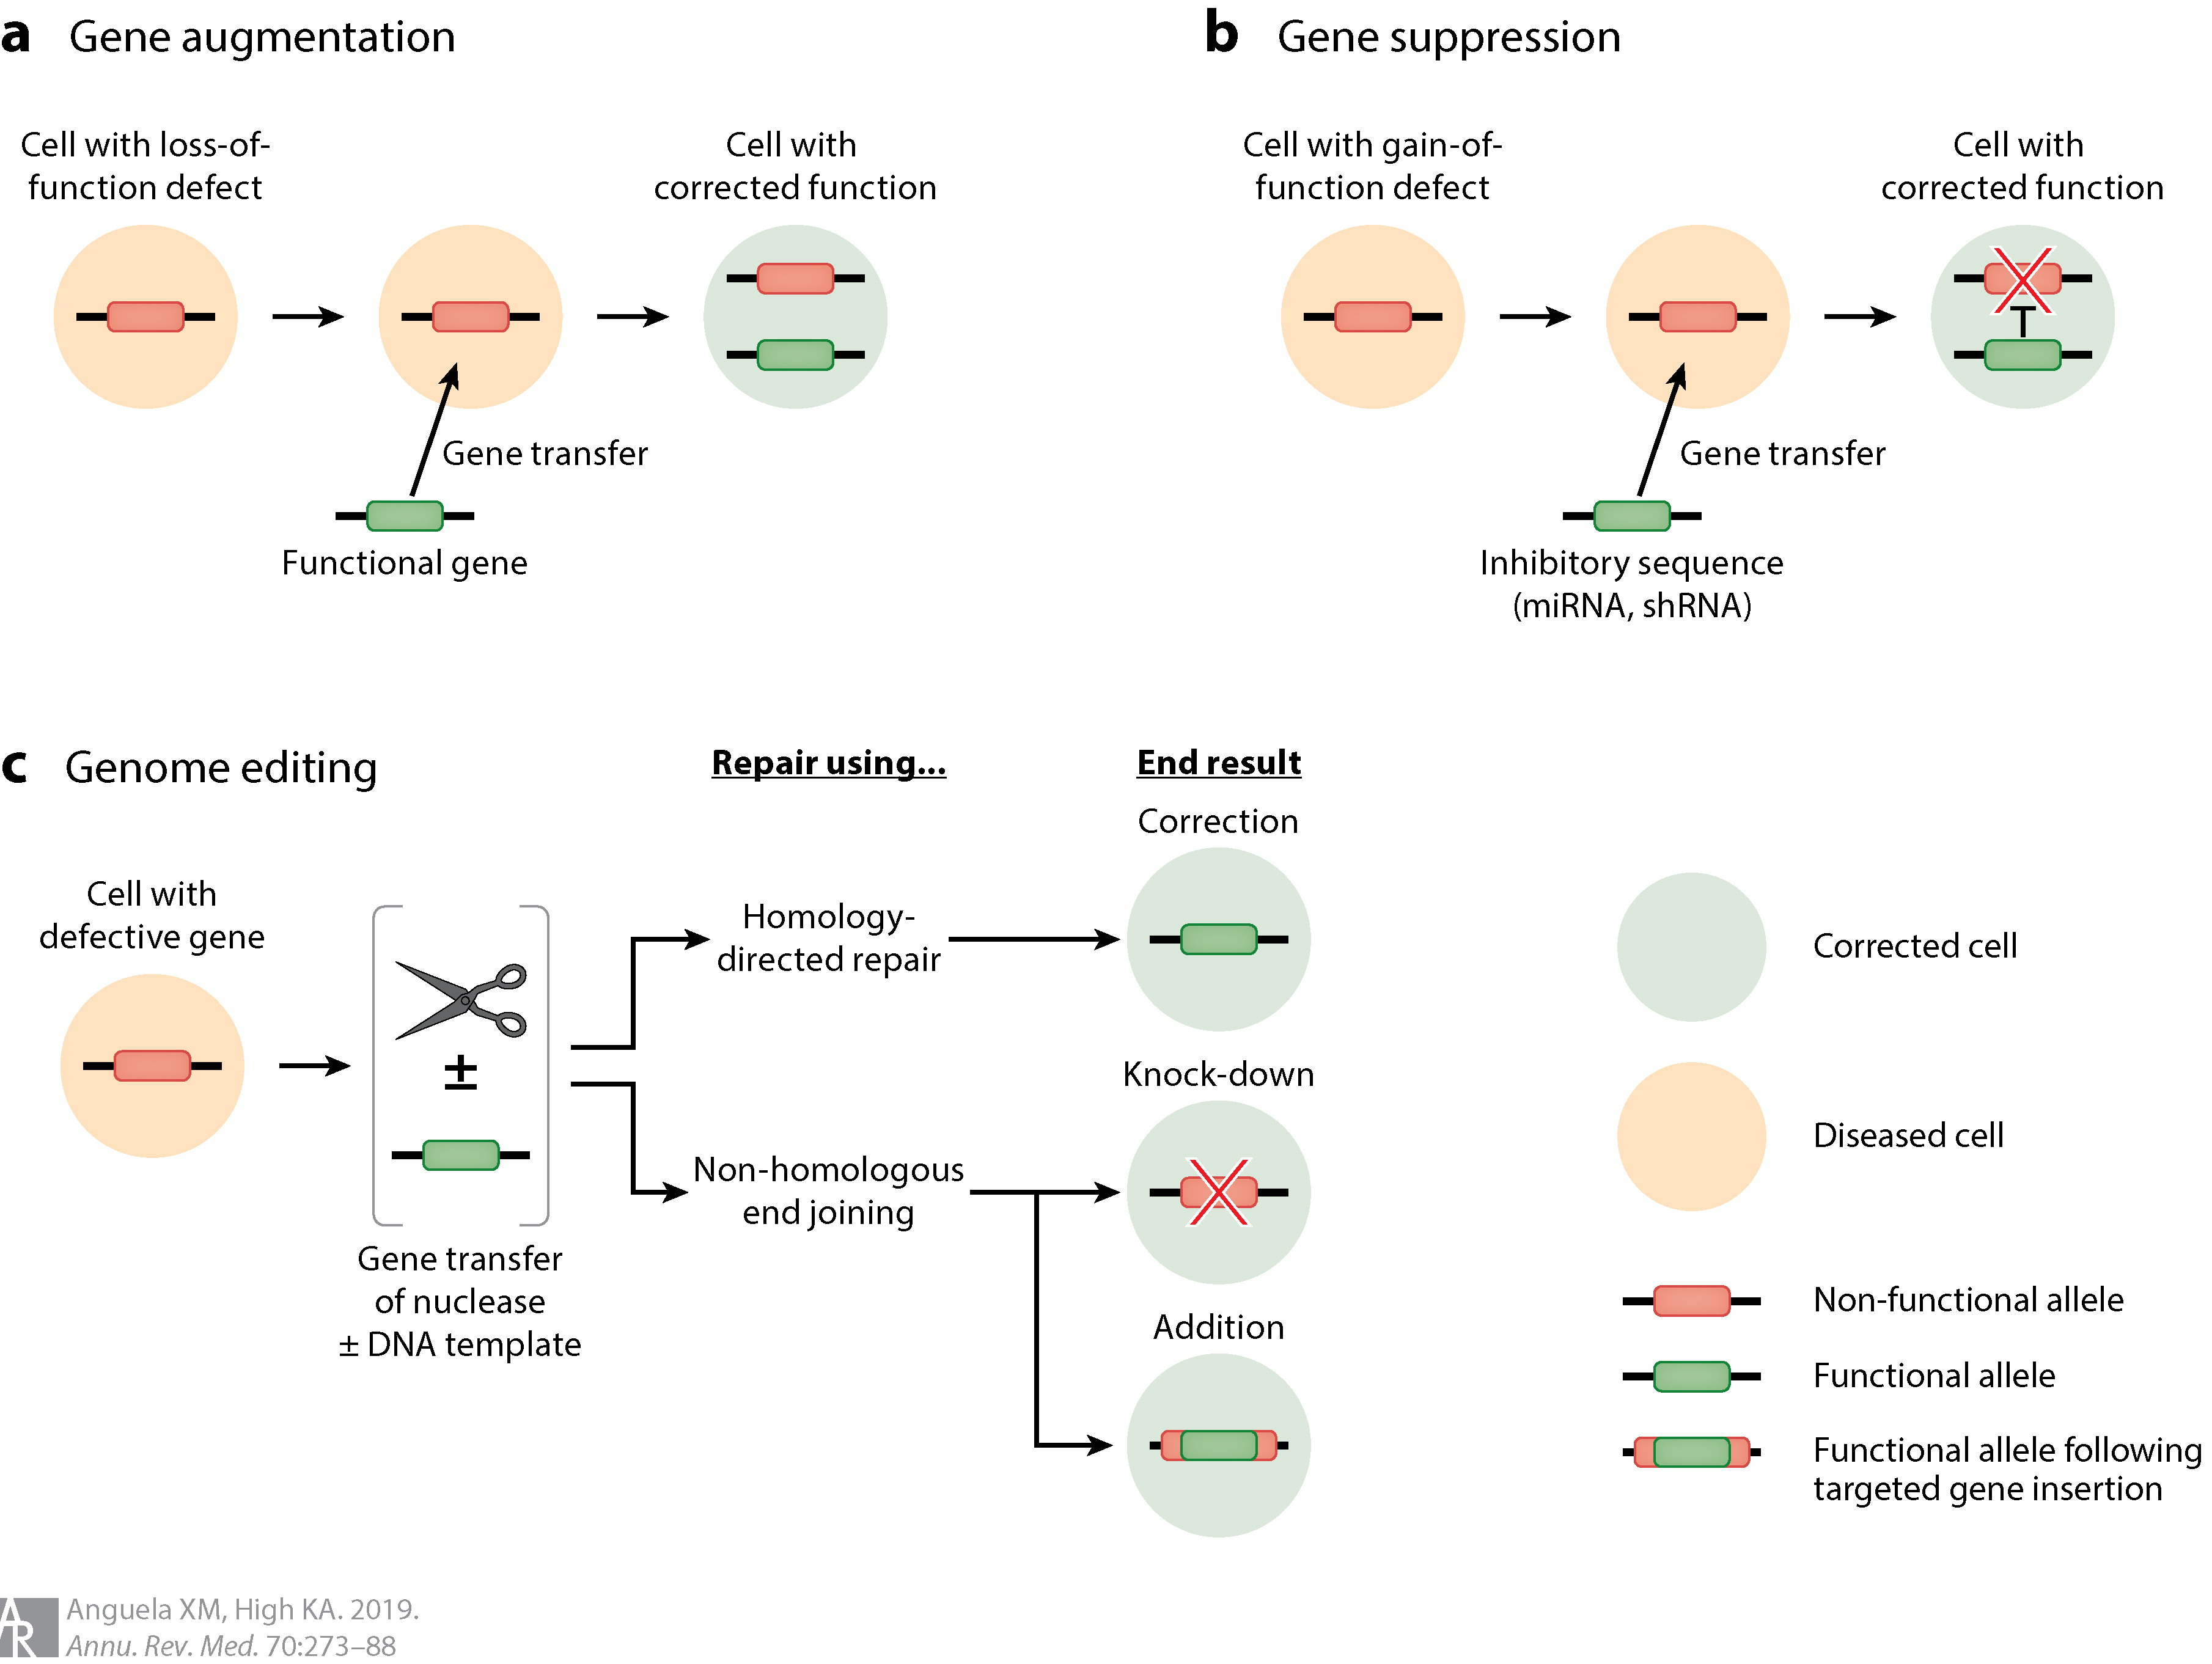
\includegraphics[width = 0.8\textwidth]{1introduction/pics/gene_therapy.jpeg}
\caption[Principles of gene therapy]{Principles of gene therapy. Reproduced from \citet{Anguela2019}.} \label{fig:gene_therapy}
\end{center}
\end{figure}

Despite the challenges posed by the development of genome editing tools, and the risk associated to them (for example the possibility of deleterious insertional mutagenesis or deleterious immune responses), at present six gene therapies have received approval in the Western world \citep{Anguela2019}, with many more undergoing regulatory review. 

One of the main problems in the development of such therapies lies in the identification of a suitable vector for the genetic material, either DNA, microRNA (miRNA) or small interfering RNA (siRNA). 
%
Delivery of free genome in solution results in poor internalisation and low therapeutic effect.
%
Thus nowadays the outlook of gene therapy research lies not only in improving specific cargos, but also in the research of appropriate vectors with low toxicity, low induced immune response and high delivery efficiency. Viruses can be used, modifying their genome to include the necessary sequence and remove the ones promoting viral replication \citep{Naldini2011,Mingozzi2011} (see Section \ref{sec:peptidic_delivery}), but synthetic vectors are now investigated for a virus-free delivery strategy. The system studied in this thesis proposes, among its other functions, to deliver genetic material into human cells.


\section{Delivery of therapeutic material}
The problem of gene delivery sets a parallel with the small drug one, introduced at the beginning of the chapter. Indeed small molecules need delivering agents to be efficiently internalised in the cells, in the same manner that genes do, and it is known that some barrier (such as the Blood Brain one) are more selective in the classes of molecules they allow to permeate \citep{Pattni2015, Krol2012}.

To reach the aimed organ, therapeutic molecules must be compatible with the different cellular environments they cross, but be preferentially retained, and act only on the ones they are designed for. This implies a subtle balance between an invasive activity on one side, and mimesis on the other, to minimise the possibility that the compound is recognised as dangerous and disposed by the immune and reticuloendothelial systems.

For the above reasons, research has focused on developing systems to assist the delivery of drugs. A mimetic carrier can not only improve delivery, but also be designed to selectively bind to particular tissues, or to trigger the drug release after a delay in time, or only upon changes in environmental variables (for example pH), to reduce drug concentration in non targeted regions. A stand alone field of research has then focused on the development of delivery vehicles irrespective from the quest for new drugs. The optimised products of the two separate efforts can then be paired according to the condition to address, to give a successful therapy.

At present, many molecules have been employed to build drug vehicles, both organic and inorganic, to offer a range of different physico-chemical characteristics useful to target different cells \citep{Hughes2005}. Inorganic materials, such as metal nanoparticles or carbon nanotubes, are in experimental phases and hold promise for promoting sustained drug release \citep{Boisselier2009,Depan2011}. Polymers, again inorganic compounds, have  instead been employed as drug eccipients in an extensive way so far \citep{Lammers2009,Liechty2010,Nicolas2013}.

The use of organic molecules instead aims at mimicking the materials present in the body, such as lipids, DNA and peptides, in an effort to reduce toxicity and favour the internalisation of the vehicle in the target cells. In particular, lipids have been widely employed for the delivery of both soluble and insoluble drugs thanks to their amphihpatic structure \citep{Pattni2015paper,Jain2017,Yingchoncharoen2016,Bunker2016}. DNA scaffolds instead are a novel tool still at the experimental stage which have been proven successful in delivering anticancer agents \citep{Zhang2014, Jiang2012}. 

But peptides are the focus of this work, and these molecules prove once more they can have functions beyond the ones they are naturally designed for. In the next paragraph we elucidate some rationale and examples of how peptide can be tuned for assembly and thus the needs of drug delivery.

%We briefly list them to point out the variety and exoticity of structures which are useful, sometimes unexpectedly, to the medical world, and we then focus on peptidic delivery vehicles: once more this class of molecules can offer a solution to a therapy-related task.

%\paragraph{Inorganic materials for small drugs delivery}

%Many inorganic compounds have been used to transport drugs or to enhance their biocompatibility. Metal nanoparticles, especially golden ones, can be customised in shape and size (down to a 10 nm radius) and coat the compound of interest. They can be optically tracked inside the body, and can be thermally stimulate to trigger drug release \citep{Boisselier2009}. To enhance their mimesis, they are coated with biologically active moieties \citep{Singh2018}, but there are mixed evidence about their toxicity \citep{Boisselier2009}, so that up to now only a few golden nanoparticle compounds have made to the clinical stage.
%%
%Carbon nanotubes are another inorganic material used for biomedical applications thanks to their high loading efficiency. This is due to their high surface area and easy interaction with biomolecules through van der Waals forces, $\pi$-$\pi$ stacking or hydrophobic effect \citep{Erol2017}. They too can be conjugated to extra organic groups to increase their biocompatibility and have potential for targeted drug release upon change in environmental pH \citep{Depan2011}.
%%
%Finally, polymers are already a well validated drug eccipient. The most notable example is Polyethylene glycol (PEG): thanks to its high hydrophilicity, it is widely used to coat structures (e.g.\ inorganic nanoparticles) which in turn carry a drug \citep{Lammers2009}, or as a stand alone carrier with high drug payload \citep{Liechty2010}. As each constituent monomer can be either hydrophilic or hydrophobic, polymers can be engineered to assemble in different structures, to swell slowly in water triggering a sustained drug release \citep{Nicolas2013}, or to undergo sol-gel phase transition upon specific changes in the environment \citep{Liechty2010}.


%\paragraph{Organic materials for delivery: lipids and DNA} \label{sec:organic}
%
%A somehow opposite approach for designing drug vehicles consists in using molecules similar to the ones present in the body, such as lipids, DNA and peptides, in an effort to exploit available biocompatible materials and reduce toxicity \citep{Yoo2011}.
%
%Many lipids are approved as delivery agents for cancer and infection drugs \citep{Pattni2015paper, Jain2017}. Usually taken from the biological lipidome, they can include also synthetic molecules, which help tuning the release and increase the robustness to degradation \citep{Yingchoncharoen2016}.
%%
%Being amphiphatic, lipids can encapsulate efficiently both hydrophobic or hydrophilic drugs, arranging respectively in micelles (monolayer spheres with the hydrophobic tails facing the interior) or in liposomes (bilayer spheres with a water filled core) \citep{Bunker2016}.
%
%DNA scaffolds are instead a novel tool: DNA origami is nowadays an established technique to build three dimensional customised solids with nanometric precision \citep{Linko2015}. When transporting a drug, they can trigger a delayed release of the content \citep{Douglas2012} and have been proven successful in delivering anticancer agents \citep{Zhang2014, Jiang2012}. However, as their stability is very sensitive to different cellular environments and they have high production costs, they are yet to constitute a viable class of carriers so far.


\subsection{Peptidic scaffolds} \label{sec:peptidic_delivery}
Another widely used and trustworthy mimetic vehicle comes, quite surprisingly, from the world of pathogens: viruses have co-evolved with humans, to be able to penetrate into cells where they complete their reproductive cycle \citep{Lobo2009}. Therefore their capsid, the peptidic shell encapsulating the viral genome, is highly suitable for cell penetration. The first application sought historically was to employ genome-free viruses to stimulate the natural immune response against the respective genome-loaded ones, creating viral vaccines - similarly to how inoculation of dead bacteria counteracts their infections \citep{Lauer2017}.
Later in the history, their potential as cargo carrier was pursued modifying the original genetic material to include sequences beneficial for the host cell, and inactivate their duplication \citep{Daya2008}.
%
Since then, many efforts have focused on synthesising in vitro gene-free capsids, either as they appear in nature \citep{Wu2009} or designing artificial building blocks which assemble in so called Virus-Like particles (VLPs) \citep{Schoonen2014} aimed at triggering a lower immune response (Figure \ref{fig:intro}, i).
%
Similarly to other delivery vehicles, the surface of VLPs can be functionalised with additional molecules to improve the target selectivity and biocompatibility, while the peptidic scaffold grants robustness to the structure. VLPs loaded with drugs can be tuned for an efficient intra cellular release \citep{Ma2012}.

A step further in engineering peptidic structures is the design of self-assembling functional blocks from first principles. Indeed, self-assembling peptides can form nanostructures ranging from nanoparticles to nanotubes, nanofibers, nanorods and hydrogels \citep{Fan2017}.
%
The variety of amino acid available makes peptidic structures compatible with both hydrophilic and hydrophobic drugs, according to their amino acid composition \citep{Ma2012}.
%
The peptidic self-assembly is modulated by the peptide length and its hydrophobic or hydrophilic character, given by its amino acid composition: simple phenylalanine dipeptides (Figure \ref{fig:intro}, j), inspired from a pathogenic self-assembly pathway, were shown to assemble in a multi-scale process into nanotubes able to load drug molecules \citep{Silva2013}. The relatively small diphenylalanine building block is nevertheless complex as it bears two charged termini (as the process is observed at neutral pH), and two aromatic hydrophobic rings, so that the dipeptide is driven towards assembly by the hydrophobic forces acting on the phenylalanine side chains and the complementary charges of the termini.

In a different approach, longer sequences (which organise spatially in well studied $\alpha$-helical or $\beta$-sheet secondary structures) can be employed to guide the assembly at the tertiary structure level (see some examples in Figure \ref{fig:amp_structure}).
%
This knowledge is possible as proteins are a fundamental component of the human body and as such an updated database of their structure is available (the Protein Data Bank \citep{PDB}) and can be queried to understand how small peptides hierarchically assemble into larger units.
%
Finally, the vast literature on their interactions with membranes, cell receptors and in general biological components, can inspire the design of building blocks sensible to particular triggers within the body. From this background, the outlook of protein design often goes in the direction of synthesising exotic, non natural geometries for multifunctional materials \citep{Yeates2019,Malay2019}.


\section{Closing the circle: an antimicrobial drug delivery vehicle}

Twice in this introduction peptide design has been brought to the reader's attention. First, it can produce antimicrobial peptides with improved potency and/or selectivity, and/or reduced toxicity. Second, it can engineer self-assembling building blocks for the formation of delivery scaffolds. As design is not bound to natural rules, it can foresee and imagine multifunctional materials which are not observed in nature. In particular, the question arises whether it is possible to engineer peptides able to perform both an antimicrobial and a delivery function at once.

Self-assembling antimicrobial compounds would have a twofold interest for medical applications.
%
First of all, the assembly is functional to the antimicrobial activity: many AMP sequences have a weak potency, and only a high (critical) concentration can trigger the bactericidal mechanism (e.g.\ the insertion into the membrane or its lysis, see Section \ref{AMP_mechs}).
%
%Indeed, as AMPs are generally positively charged, the localised presence of many copies of a sequence enhances the local electric field and charge imbalance, which are critical to the membrane stability. 
%Thus a self-assembling sequence will enhance the local concentration which is crucial to initiate the membrane disruption.
%
Second, the assembly can perform additional delivery functions, if it is able to either organise in a tailored structure (for example a capsule able to host a drug), or to co-assemble with the cargo of interest.

Out of all the possible applications, the most promising is perhaps the use of such vehicles to deliver drugs to treat metabolic or genetic diseases: while the cargo tackles a defect of the host system, the vehicle can counteract the proliferation of bacteria. This is particularly important when the host immune response is weakened and normally harmless infections can spread and cause damage.
%
As such, the cargo is not bound to be a small molecule, as long as it can effectively co-assemble with the peptidic carrier. As mentioned in the previous section, gene therapy is also an actively expanding field which looks with interest at the development of vehicles. Given that viruses have been the first choice for DNA/RNA delivery so far, peptidic carriers seem their natural evolution.

Given the above premises, it is evident the importance of pursuing the research on novel multifunctional peptidic materials.
%
As mentioned when discussing AMPs design, to better understand these systems, each of them must be characterised by itself, as a generalised knowledge is still lacking.
With this aim, this thesis proposes to elucidate the behaviour of a specific synthetic self-assembling peptide, suitable for antimicrobial activity and gene delivery strategies.
%
Its characterisation will complete the knowledge on its mechanisms of action and complement the general information already known on the class of such functional building blocks. This is crucial to engineer new synthetic blocks with improved characteristics, either regard their antimicrobial activity, assembly performances, or tailored cargo delivery.


\subsection{The capzip molecule} \label{sec:capzip}

\begin{figure}
\begin{center}
\subbottom[]{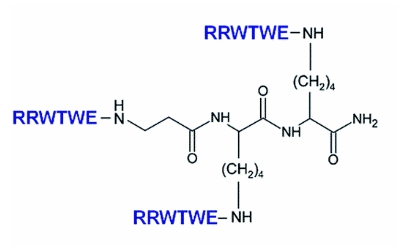
\includegraphics[width=0.4\linewidth, align = c]{1introduction/pics/triskelion_chem} \label{fig:capzip_chem}} \hspace{0.5cm}
\subbottom[]{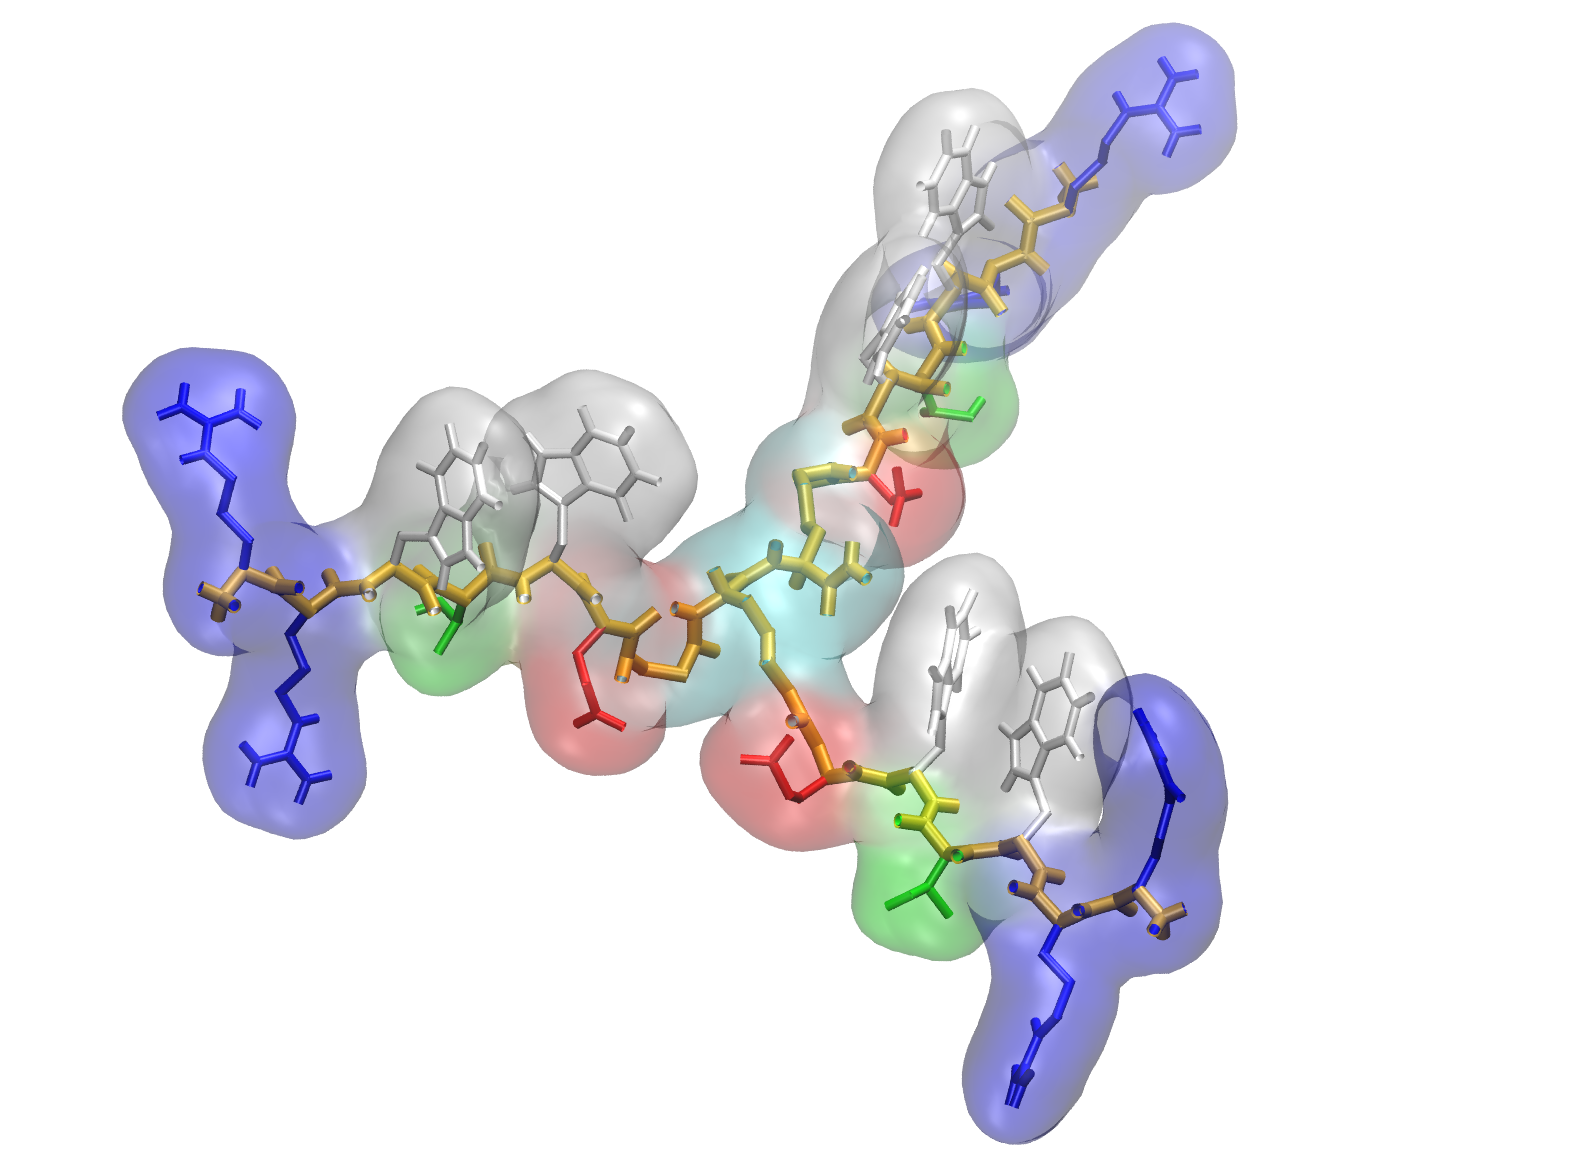
\includegraphics[width=0.45\linewidth, align = c]{1introduction/pics/triskelion_surf} \label{fig:capzip_surf}}
\caption[Cazip molecule]{Capzip molecule: (a) scheme of chemical formulation, reproduced from \citet{Castelletto2016}; (b) 3D bonds representation: backbone in yellow, amino acids side chains colored by residue type (blue positive, green hydrophilic, white hydrophobic) [VMD software \citet{HUMP96}].} \label{fig:capzip}
\end{center}
\end{figure}

The molecule capzip \citep{Castelletto2016} (Figure \ref{fig:capzip}) has been designed to perform the functions mentioned above at once. To recapitulate, the properties it possesses are:
\begin{enumerate}
\item assembly into nanoscale virus-like capsules with and without nucleic acids. This ensures that the vector can autonomously form and thus there is flexibility in the choice of the cargo;
\item antimicrobial activity of the molecule itself and of the capsule on a time scale useful for therapeutic applications;
\item promotion of gene transfer into mammalian cells when the peptide is co-assembled with the RNA strands, without causing cytotoxic and haemolytic effects.
\end{enumerate}

Its design aimed at building a template structure of minimal complexity, in order to synthesise only a short sequence. Arguably, short sequences are flexible in their assembly, as they do not rearrange into defined secondary structure: it is thus even more important to understand them and prove whether also small blocks can form ordered architectures.
%
To satisfy the short sequence criterion and the required properties of the assembly, two design principles emerged: first the employment of a non-linear structure, and second the use of a template antimicrobial sequence which is short and has proved efficacy.

There is indeed some evidence suggesting that the branching of short peptidic sequences without secondary structure tunes their three dimensional assembly \citep{Gudlur2012,Breger2017,Zhao2018branch}. Moreover, many viral structures have a 3- or 5-fold symmetry at each of their vertices \citep{Schoonen2014}: reproducing this, albeit in a different structure, is likely to improve its assembly properties.
%
for these reasons, a short peptidic scaffold constituted by a $\beta$-Alanine and two Lysins which can host other peptidic branches has been engineered as core of the capzip molecule.

Regarding the second principle, the antimicrobial sequence selected has been derived from the AMP bovine lactoferricin, which is in turn a portion of the Lactoferrin protein, and is six amino acids long (see next paragraph).
%
Three copies of it are covalently bonded to the N-terminus of the scaffold sequence and to the nitrogen atom of the Lysin side chains (Figure \ref{fig:capzip_chem}).
%
As AMPs are usually cationic, and indeed the overall structure has a $+6e$ charge at physiological pH, the co-assembly with anionic RNA sequences is arguably naturally inherited by the molecule.


\paragraph{Lactoferrin} Lactoferrin is an iron binding protein present in milk (in which it is most abundant, hence its name), saliva and other secretions, as well as in leukocytes (Figure \ref{fig:blf} shows the bovine homologue of the human protein).
%
It works as an iron binder and provides a natural defence against bacteria and fungi \citep{Sanchez1992,Arnold1977,Arnold1980,Kirkpatrick1971,Jahani2015}, constituting a first defence for infants.

\begin{figure}
\begin{center}
\subbottom[]{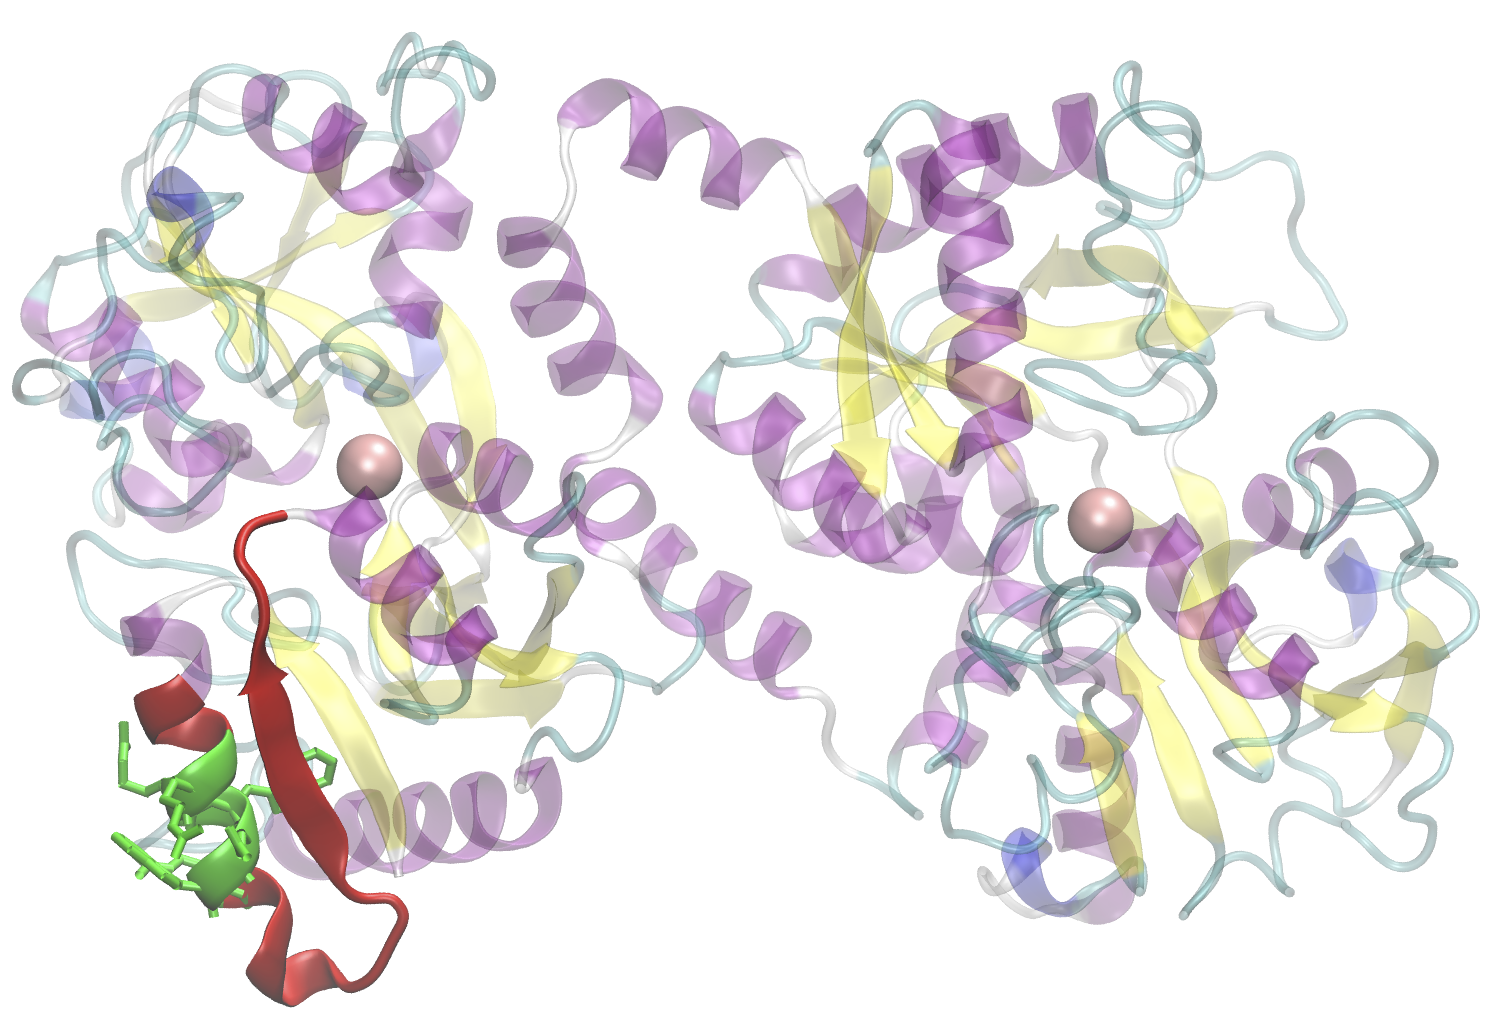
\includegraphics[width=0.4\linewidth, align = c]{1introduction/pics/blf} \label{fig:blf}} \hspace{0.3cm}
\subbottom[]{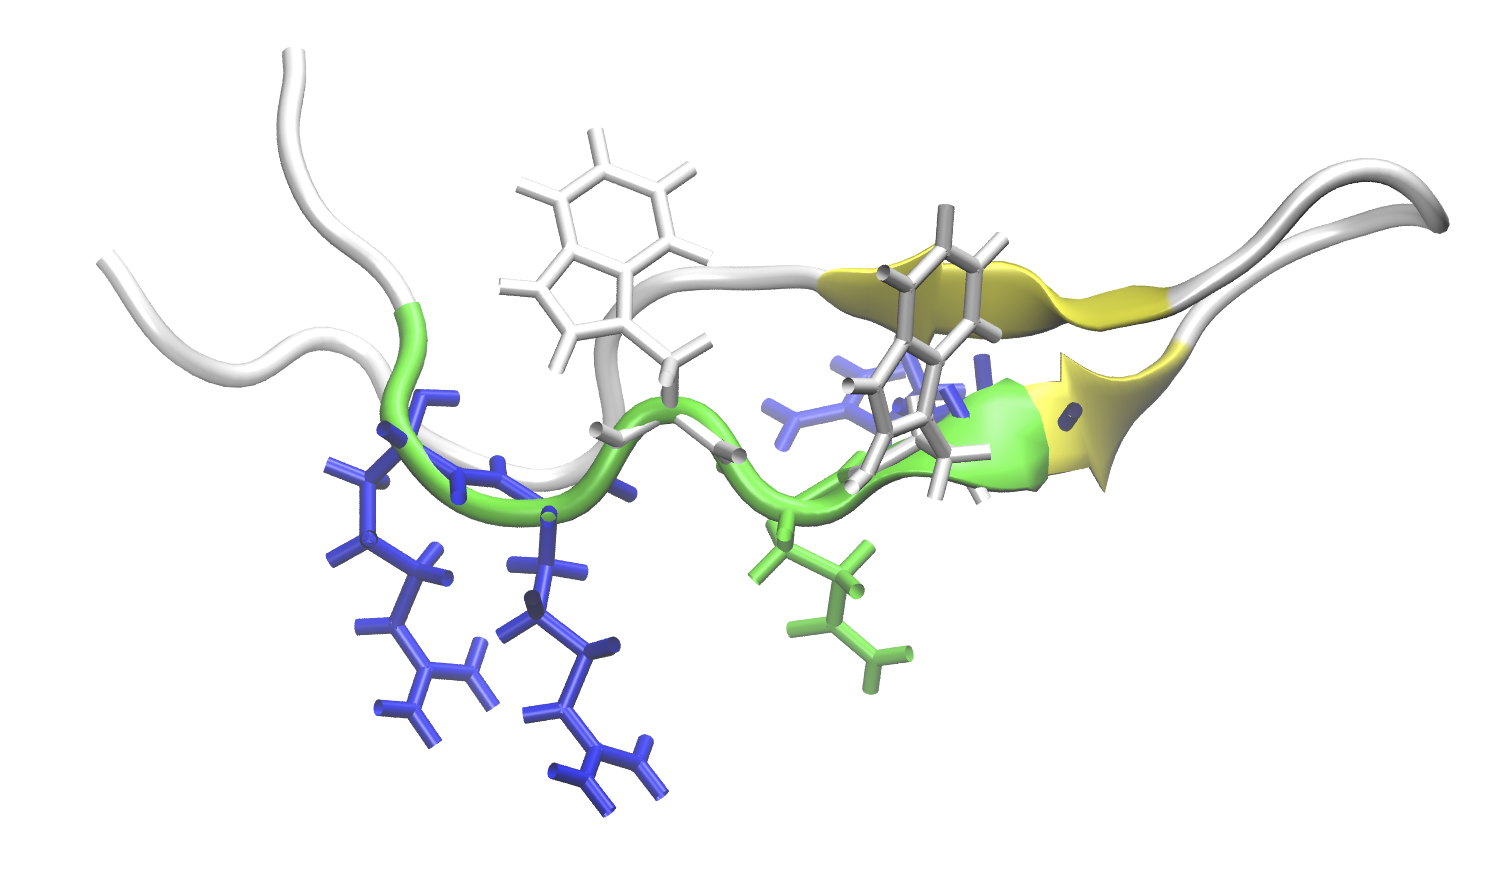
\includegraphics[width=0.4\linewidth, align = c]{1introduction/pics/lfc} \label{fig:lfc}}
\caption[Lactoferrin and lactoferricin proteins]{(a) Bovine lactoferrin protein (PDB code 1BLF): transparent cartoon representation, colored by secondary structure. In red is highlighted the portion of sequence corresponding to lactoferricin. In green, the 6 amino acid antimicrobial sequence. In pink spheres the iron ions. (b) Bovine lactoferricin protein (PDB code 1LFC); cartoon representation, colored by secondary structure. In green, and in bond representation color coded by amino acid type, the 6 amino acid antimicrobial sequence. [VMD software \citet{HUMP96}]} \label{fig:blf_lfc}
\end{center}
\end{figure}

Lactoferrin contributes to bacterial suppression in several ways. At present, its known modes of action fall in three categories: first, thanks to its iron sequestering capabilities, it removes essential substrate required for bacterial growth \citep{Farnaud2003}; second, it is implicated in the stimulation of different immunological cells (killer cells \citep{Shau1992}, polymorphonuclear leukocytes, and macrophages \citep{Gahr1991}); finally it interacts with bacterial membranes and binds to the lipopolysaccharides of the bacterial wall, oxidising them and affecting the membrane permeability with consequent cell lysis \citep{Farnaud2003}.
The peptide fragment responsible for binding lactoferrin to the bacterial membrane, named lactoferricin (Lfcin), has been identified near its N-terminus and found to have a more potent bactericidal effect than intact lactoferrin on a wide range of bacteria \citep{Gifford2005,Bellamy1992,Tomita1994,Wakabayashi1996} (Figure \ref{fig:lfc} shows the bovine homologue of human Lfcin).
%
Similarly, an even shorter subsequence of human lactoferricin has been proven effective against bacteria as it depolarises the cytoplasmic membrane decreasing the pH gradient \citep{Aguilera1999}.

The bovine homologue of lactoferricin (LfcinB, Figure \ref{fig:lfc}, PDB code 1LFC) has often a higher bactericidal potency than its human counterpart \citep{Cochran2001} and therefore has been more extensively studied. It is a 25-amino acid sequence which adopts a helical conformation in the full structure but, once isolated, crystallises in a $\beta$-hairpin with a disulfite bridge nearby the terminals which stabilises the fold, but was shown to be not essential for the bactericidal activity \citep{Cochran2001}.
%
In solution, it adopts a flexible conformation, as assessed by NMR experiments \citep{Hwang1998}. 
%
Further experiments on LfcinB subsequences identified a shorter antimicrobial core, constituted by the six amino acids RRWQWR \citep{Schibli1999}. This core presents a characteristic Tryptophan zipper motif WQW, which appears very often in nature in $\beta$-turns and $\beta$-sheets, paired to another copy of the same motif \citep{Cochran2001} so that Tryptophan rings from facing strands are packed tightly against each other in an alternated way (Figure \ref{fig:trp_zip}).

\begin{figure}
\begin{center}
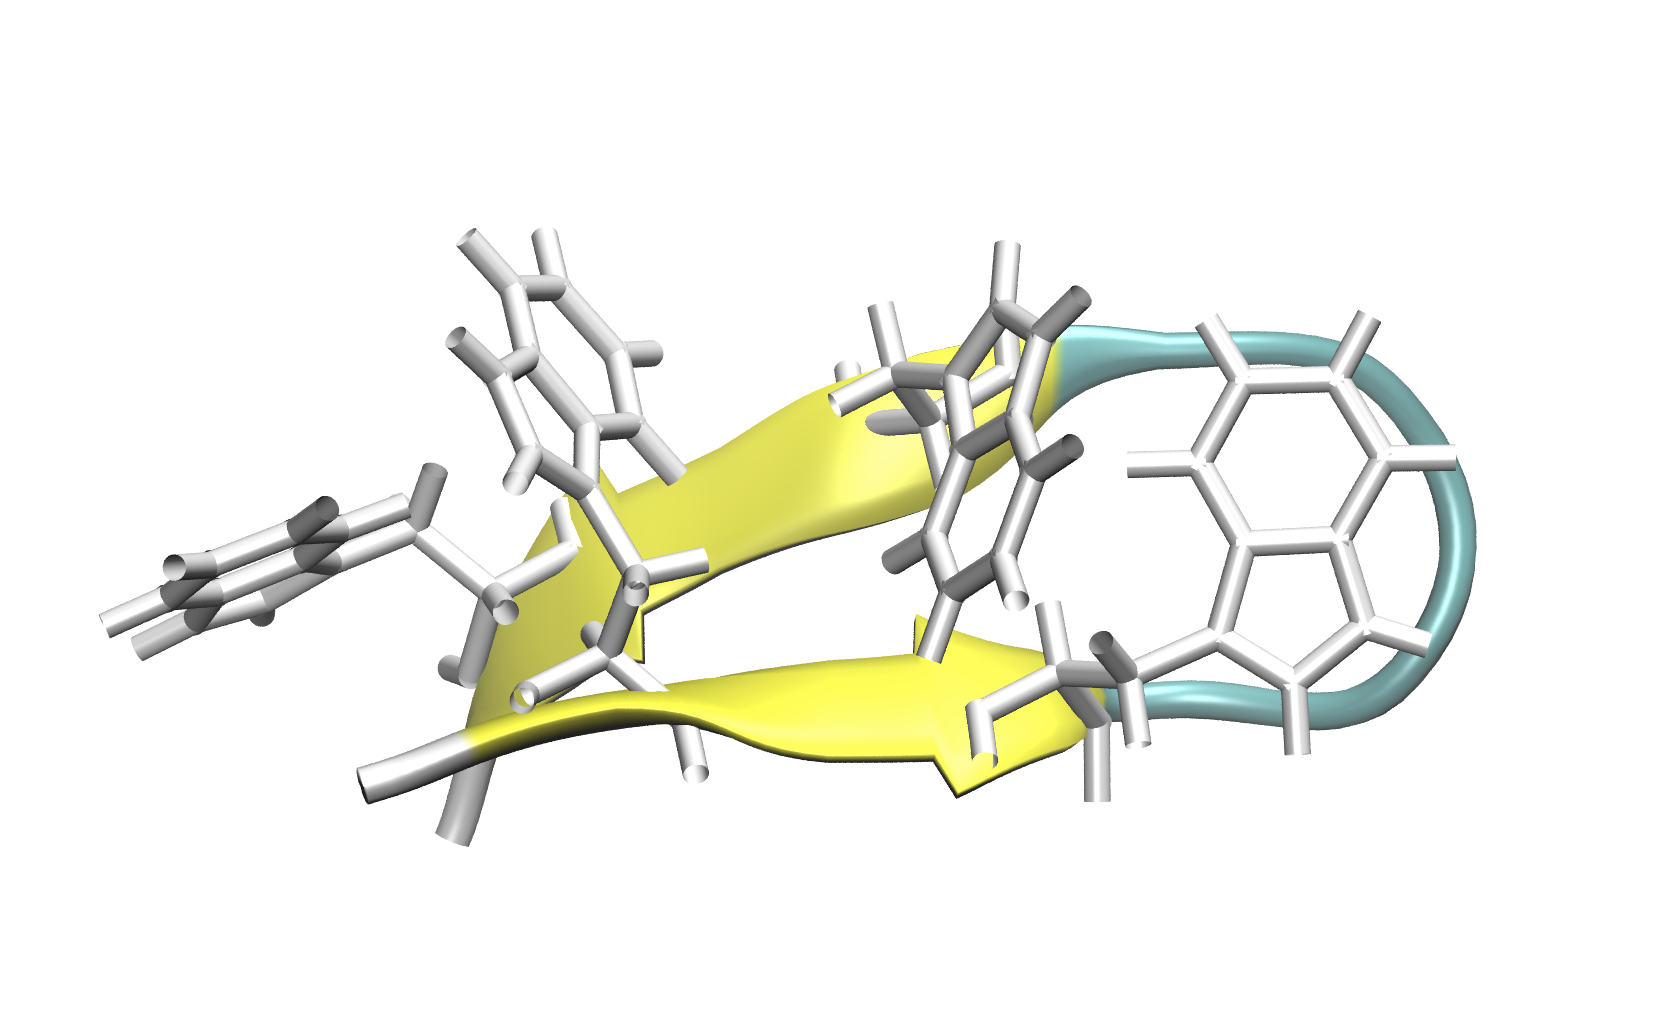
\includegraphics[width=0.5\linewidth]{1introduction/pics/trp_zip}
\caption[TRyptophan zipper 1LE0]{Example of Tryptophan zipper hairpin (PDB code 1LE0). Cartoon representation, colored by secondary structure, and bond representation for Tryptophan residues. [VMD software \citet{HUMP96}]} \label{fig:trp_zip}
\end{center}
\end{figure}

The six amino acid sequence contains both charged and hydrophobic residues, in line with the usual composition of antimicrobial peptides. Accordingly, its antimicrobial action is likely derived from the interaction with biological membranes through charge recognition first and aromatic rings insertion in a second moment.

To further elucidate this mechanism, several experimental investigations have been carried on, both on LfcinB and its subsequences. The binding of its antimicrobial core to sodium dodecyl-sulfate micelles was studied \citep{Schibli1999}, suggesting a favourable interaction of the aromatic residues with the micelles surface.
%
Similar experiments were performed on large unilamellar vesicles, constituted by lipids modelling biological membranes \citep{Nguyen2005}: ePE:ePC was chosen as a model of a mammal membrane, and ePE:ePG or ePC:ePG for a bacterial one (with PG anionic). The experiments showed preferential binding to the latter ones, based on Tryptophan fluorescence, suggesting a selective antimicrobial action on anionic membranes.
%
Additional experiments performed on other LfcinB subsequences, some of which introduced mutations \citep{Tsutsumi2012,Arseneault2010}, investigated the binding to different model membranes. However, as both the systems and the experimental conditions are slightly different each time, it is difficult to give a unified interpretation of the modes of action of lactoferricin-derived peptides.

Finally, an alanine scanning has attempted to clarify the role of each amino acid in the antimicrobial activity of the original 25 amino acid LfcinB peptide \citep{Strom2002}. The results suggested a binding function for the Tryptophan residues, in line with one of the roles Tryptophan assumes in antimicrobial sequences \citep{Chan2006}.
%
Another possible role, however, involves its propensity to form hydrogen bonds, in which case the residue would position itself at the interface between solution and membrane, rather than inside the latter, which happens when Tryptophan has a binding role \citep{Chan2006}.

\paragraph{The designed block}
From the active core of LfcinB (of sequence RRWQWR), a mutated sequence was obtained to comply the design criteria of a self-assembling building block. Two mutations were introduced to favour the assembly of arms belonging to different molecules in an antiparallel fashion. Specifically, given that the original sequence is found in a $\beta$-sheet (at least in the crystal lattice) facing a non-homologous one, the mutations aim at promoting  $\beta$-sheet formation when two pairs of the \emph{same} sequence are in proximity. Therefore, the Glutamine residue and the C-terminal Arginine of the lactoferrin motif were replaced with Threonine and Glutamic acid to have a self-complementary sequence RRWTWE: the pairing is promoted by the attraction of opposite charges at the ends of the sequence.
%
Three copies of this sequence were thus covalently bonded to the scaffold as described previously (Figure \ref{fig:capzip_chem}), to obtain a self-assembling molecule hosting multiple copies of an antibacterial sequence.

An additional layer of complexity has been added in the experimental investigation by synthesising a capzip molecule formed by D-amino acids only. The rationale behind this choice lays in the enhanced stability of D-peptides against proteolysis and their possibly low immunogenicity \citep{Uppalapati2016,Arranz-Gibert2018,King1994}, while the fold of the final product remains similar to its L- version.
%
Moreover, as antimicrobial peptides bind to membrane rather than dock to a specific protein, their D-epimer is likely to retain the activity of the L- counterpart \citep{King1994,Bland2001}.
%
This approach opens a new landscape in the field of peptide design, as it virtually multiplies the space of sequences available by a factor $2^N$, with $N$ the length of the sequence selected.


\subsection{A viable systems: experimental background and question}
A set of experiments has been performed to verify that capzip had the characteristics it was designed for. The results obtained on the molecule have been published in \citet{Castelletto2016}, while more recent investigations extended and consolidated the previous findings \citep{Kepiro2019}.

\begin{sidewaysfigure}[p!]
\begin{center}
\subbottom[]{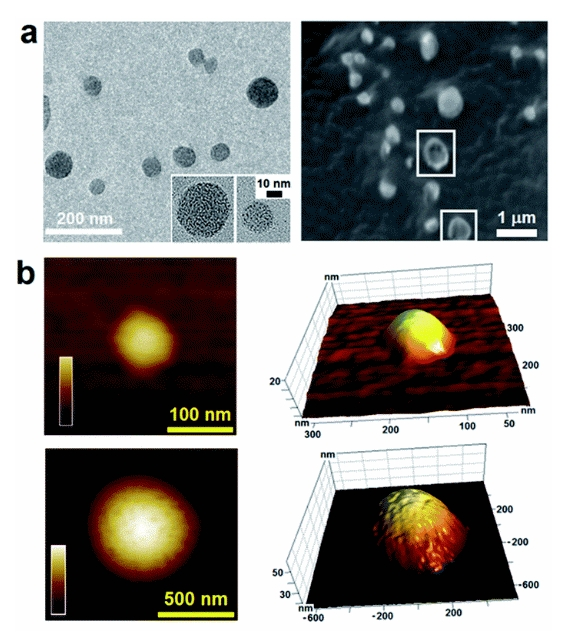
\includegraphics[width=8cm, align = c]{1introduction/pics/paper_npl_2} \label{fig:afm_L}} \hspace{0.3cm}
\subbottom[]{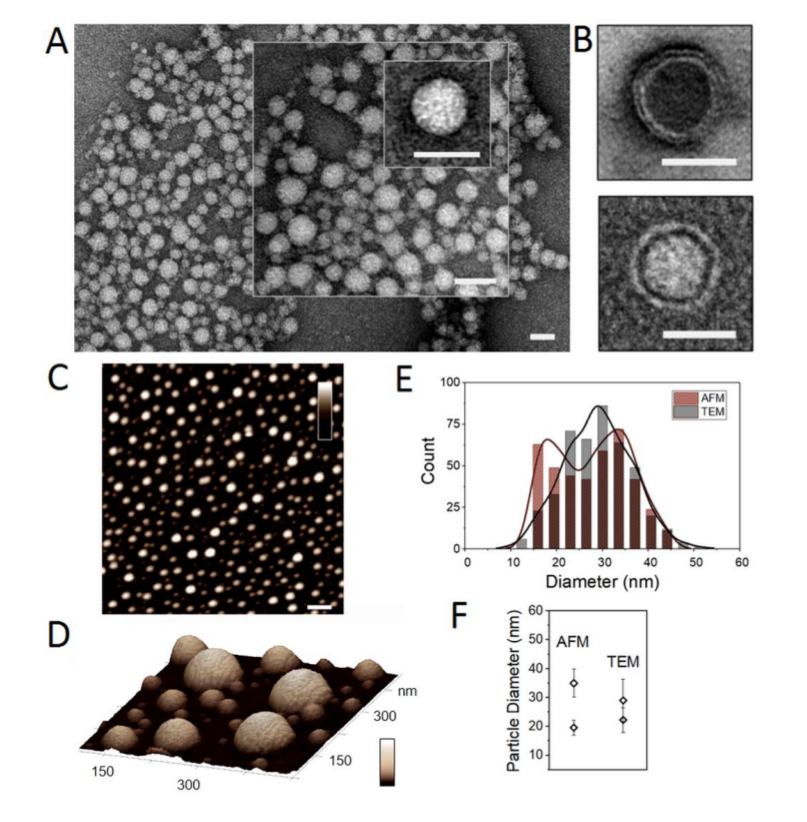
\includegraphics[width=8.5cm, align = c]{1introduction/pics/Dcapzip_afm_tem} \label{fig:afm_D}}
\caption[Miscoscopy experiments results on capzip capsules]{(a) TEM (top, left) and cryo-SEM (top, right) images of assembled capzip capsules. Collapsed ones are highlighted by white squares. In-air AFM topography of capsules and their 3D representations (middle - colour bar 20 nm and bottom - colour bar 60 nm). Reproduced from \citet{Castelletto2016}. (b) A: TEM images of assembled D-capsids (scale bars 50 nm). B: higher resolution TEM images of individual collapsed capsids (scale bars 50 nm). C: topography images of D-capsids obtained on a mica substrate by in liquid AFM (colour/height - and scale bars are 60 nm and 200 nm, respectively). D: 3D representation of D-capsids (height bar 65 nm). E: size distributions and dominating sizes of D-capsids by AFM and TEM. F: average sizes of dominating populations of D-capsids. Reproduced from \citet{Kepiro2019}. For both (a) and (b), assembly conditions: 100 μM peptide, pH 7.4, 10 mM MOPS, 20 ̊$^{\circ}$C, overnight (15 hours).} \label{fig:exp_structure}
\end{center}
\end{sidewaysfigure}

\paragraph{Experimental results} First, the assembly ability has been tested: the peptide (L-version) did not assemble in pure water (as verified by Dynamic Light Scattering), while in biological buffer (MOPS, 10 mM) at physiological pH of 7.4, it formed capsules with dominating size range of 20-200 nm. This was confirmed by images of the capsules obtained with multiple techniques, namely transmission electron microscopy (TEM), atomic force microscopy (AFM), and cryo-scanning electron microscopy (SEM) (Figure \ref{fig:afm_L}).
%
Analogous and more systematic investigation on D-capzip brought to similar conclusions (Figure \ref{fig:afm_D}), restricting the dominant size range from 20 to 40 nm of diameter.
%
Interestingly, some of the images collected showed ring structures, likely derived from collapsed capsules, suggesting they are hollow. 
%
Fluorescence microscopy of a capsule assembled from fluorescein labelled capzip confirmed this hypothesis, showing that the signal was coming from the walls of the structure only.

The fine structure of these assemblies appeared irregular to the resolution of the miscoscopy techniques employed and could not be fully determined. Some insight was given by Circular Dichroism (CD) spectra, which showed a profile characteristic of $\beta$-turns and contained elements of a $\beta$-sheet structure and of indole rings (minima at $\lambda \sim$ 200 nm and 214 nm) (Figure \ref{fig:exp_CD}).

\begin{figure}
\begin{center}
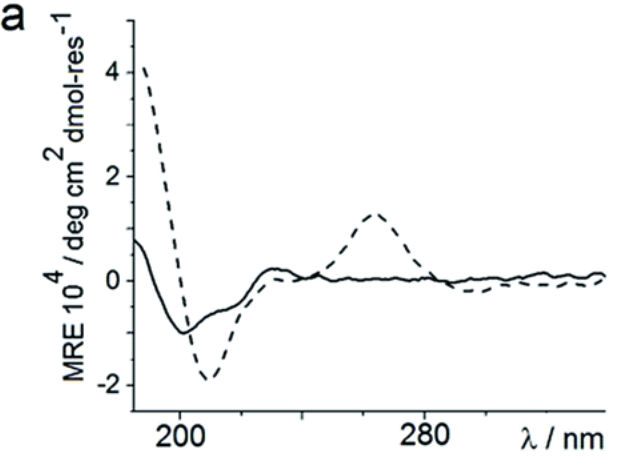
\includegraphics[width=0.6\linewidth, align = c]{1introduction/pics/CD_capzip.png}
\caption[Circular Dischroism specturm of capzip capsules]{Circular Dischroism spectra for capzip  capsules (solid line) and capzip with siRNA (30 $\mu$M, dashed line). Reproduced from \citet{Castelletto2016}} \label{fig:exp_CD}
\end{center}
\end{figure}

The assembly process was also tested and monitored in combination with small interfering RNA (siRNA) sequences. The co-assembly of a 21 base pairs duplex with the peptide showed the formation of structures similar to the ones with peptide only: CD spectra highlighted the helical signal from RNA together with the features proper of the peptide (Figure \ref{fig:exp_CD}, dashed line).
%
These co-assembled structures were tested for siRNA delivery in HeLa cells, thanks to their GPF (Green Fluorescent Protein) silencing activity: in cells expressing GFP, the delivery of such siRNA sequences would stop the fluorescent signal, up to degradation of the siRNA strands. The experiment showed that the internalisation occurred within the first hours from the transfection, suggesting an endocytic uptake (Figure \ref{fig:exp_rna}, a). The presence of the peptide enhanced the internalisation with respect to the one obtained from a pure siRNA control (Figure \ref{fig:exp_rna}, a), and was comparable with the uptake obtained with the standard transfection agent Lipofectamine\textsuperscript{\textregistered}.
%
The GFP silencing was stable over the first five hours of incubation after which the fluorescence signal decayed. 

Similar transfection experiments using a fluorescent Alexa-labelled siRNA (Eurogentec, UK) combined with D-capzip were assessed through flow cytometry assays. This method counts the number of fluorescent cells and can process thousands of them at once, giving large scale information on the efficacy of the transfection. Such assays confirmed that also D-capzip enhance the siRNA uptake in measure comparable with Lipofectamine\textsuperscript{\textregistered} performances (unpublished results).

To further quantify the level of RNA internalisation, a micro RNA (mRNA) knockdown experiment was performed on a HeLa cell line with two housekeeping genes, ACTB ($\beta$-actin, targeted) and GAPDH (reference).
%
The silencing of $\beta$-actin mRNA was detected 22 $\pm$ 2 hours after transfection. Its knockdown ``fitness" (Figure \ref{fig:exp_rna}, b) was computed relative to cells treated with siRNA alone (background) and normalised against viable cell counts. Capzip fitness was lower than Lipofectamine\textsuperscript{\textregistered} one, however cells treated with capzip remained viable longer, suggesting that capzip has little cytotoxicity.
%
The experiment was performed at neutral to positive charge ratio close to one (where each siRNA molecule has a -42$\, e$ charge and capzip a +6$\, e$ charge). Test experiments performed at higher peptide-to-siRNA ratio showed no improved uptake.

\begin{figure}
\begin{center}
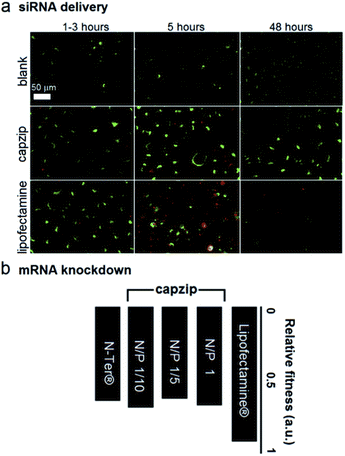
\includegraphics[width=0.6\linewidth, align = c]{1introduction/pics/capzip_delivery.png}
\caption[Capzip promoted RNA transfection]{a: fluorescence micrographs of HeLa cells expressing green fluorescent protein used as internal background fluorescence for Alexa647-labelled siRNA, at 1/5 N/P (neutral to positive) molar ratios. b: knockdown fitness of capzip and commercial Lipofectamine\textsuperscript{\textregistered} or N-TER\textsuperscript{\textregistered} (positive controls) normalised against siRNA alone (negative control) and the total counts of viable cells. Reproduced from \citet{Castelletto2016}.} \label{fig:exp_rna}
\end{center}
\end{figure}

Finally, the peptide exerted an antimicrobial function: both the L- and D- non-assembled peptides were effective against Gram-positive and negative bacteria (S. aureus, B. subtilis, M. luteus - positive - and E. coli, P. aeruginosa, S. typhimurium, K. pneumoniae - negative).
%E. coli (-)
%S. aureus (+)
%P. aeruginosa (-)
%S. typhimurium (-)
%K. pneumoniae (-)
%B. subtilis (+)
%M. luteus (+/variable)
The minimum inhibitory concentrations (MIC), the lowest concentration which prevents visible growth of the bacterium, was typical of other antimicrobial agents. This antimicrobial action extended also to cell types which are not susceptible to ampicillin (Figure \ref{fig:exp_ecoli}, B).
%
Additionally, no haemolytic effects were observed on human erythrocytes, i.e.\ the concentration required to achieve 50\% cell death compared to untreated cells (LC$_{50}$) was larger than 10 times the MIC necessary to kill most bacterial species.

\begin{figure}
\begin{center}
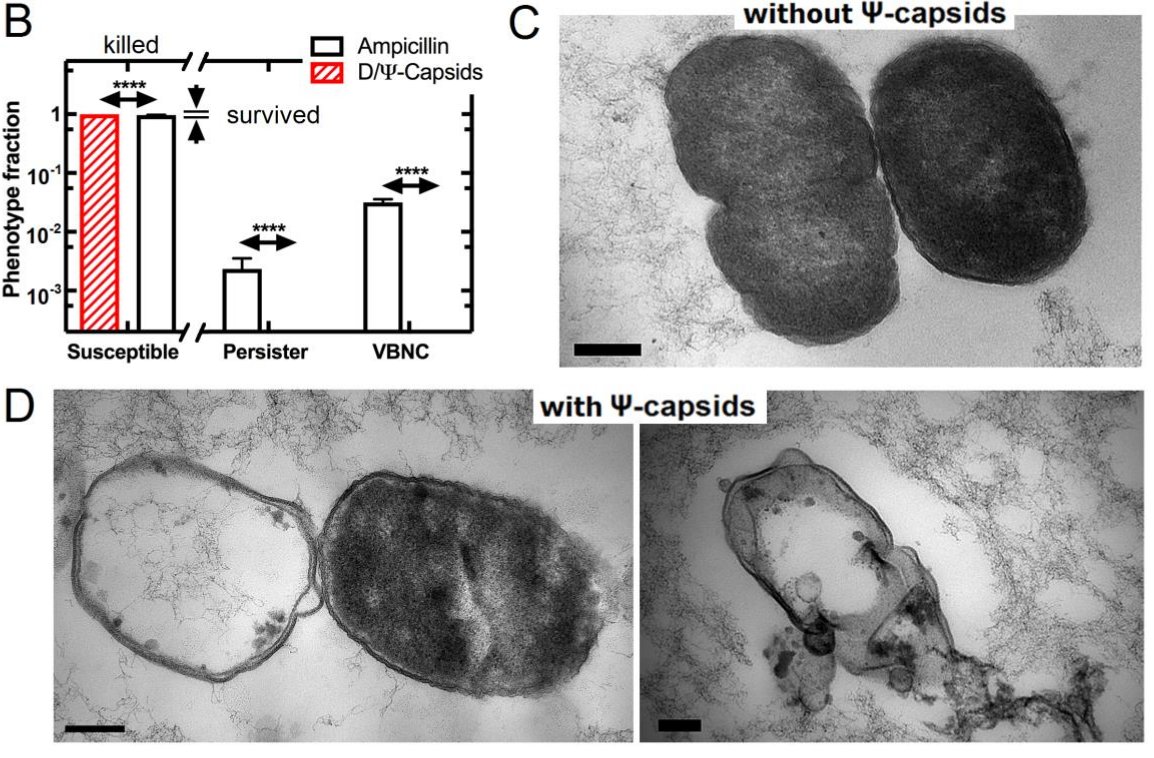
\includegraphics[width=0.8\linewidth, align = c]{1introduction/pics/ecoli_disruption}
\caption[Effect of capzip on bacterial cells]{B: E. Coli cell fractions treated with D-capsids and ampicillin (means and standard error obtained for 3332 cells hosted in 2331 independent microfluidic channels). C and D: electron micrographs of microtomed E. coli cells before (C) and after (D) treatment with D-capsids (scale bar 200 nm). Reproduced from \citet{Kepiro2019}.} \label{fig:exp_ecoli}
\end{center}
\end{figure}

To better understand the type of action capzip performs on the bacteria, electron micrographs of E. Coli cells were taken before and after the treatment. Figures \ref{fig:exp_ecoli} C and D show the membrane disruption and the leakage of intracellular material after the introduction of capzip.
%
A more detailed view of the effects of a capzip capsule on the bacterial membrane was provided by experiment on Supported Lipid Bilayer with negative total charge (mixed DLPC and DLPG, 3:1 ratio). Deposition of capsules on them created localized pores within minutes, as proven by AFM experiments repeated in time. The pore depth ranges between 1.4 and 2.2 nm, which is smaller than the radii of the capsules, but is sufficient to disrupt the structure of the membrane (Figure \ref{fig:exp_SLB}).

\begin{figure}
\begin{center}
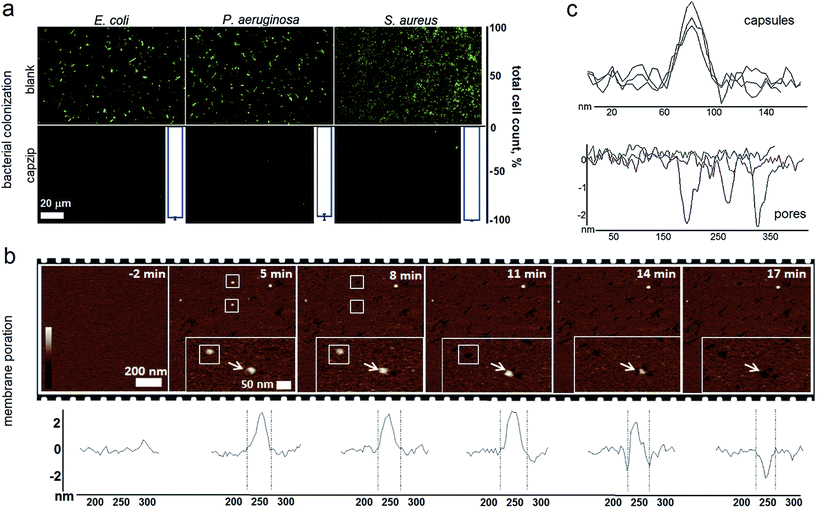
\includegraphics[width=0.8\linewidth, align = c]{1introduction/pics/AFM_on_SLB}
\caption[Capzip experiments on Supported Lipid Bilayers]{Antimicrobial activity of capzip capsules on bacterial model membranes (Supported Lipid Bilayer). (a) Confocal micrographs of stained bacterial cells after 16 hour incubations with and without capzip. White histogram bars denote total cell counts (\%) for bacterial colonization with capzip after subtracting background adhesion taken as 100\%. (b) AFM topography of SLBs during capzip incubation in solution. White boxes and arrows highlight individual capsule conversions into pores (color scale 6 nm). Cross sections show the evolution of this capsule into a pore in real time. (c) Representative cross-sections of capsules and pores. Reproduced from \citet{Castelletto2016}.} \label{fig:exp_SLB}
\end{center}
\end{figure}

Finally, to prove the viability of capzip as antimicrobial agent in vivo, it was used to counteract methicillin-resistant S. aureus (MRSA) infections in G. mellonella larvae. The particular bacterial strain used was susceptible to vancomycin, which could be used as control: the larvae treated with capzip showed survival rates significantly higher than the untreated control, and comparable to those treated with high doses of vancomycin \citep{Kepiro2019}.


%MANCA: microfluidic results

\paragraph{Open questions} Despite the success of the experiments mentioned above, there is much information still to be uncovered on the precise action of such peptide. 
%
Specifically, both the assembly process and the antimicrobial mechanisms contain some unknown.

Regarding the former, it is important to understand (a) which amino acids or sub-structures allow the pairing of molecules, (b) whether such pairing is specific or not, (c) how reversible it is, and (d) how rigid the final structure is.
%
Regarding the latter, it must be highlighted (a) what moieties in the membrane the peptide binds to, and (b) how this binding affects the full membrane structure.

Finally, as there is evidence that the assembled molecule is a more powerful antimicrobial compound than the single one, it is interesting to understand whether any cooperative action is taking place, or the enhanced antimicrobial power of the assembly is due only to the localised higher concentration of antimicrobial sequences.

Even if further experiments or future improvements in the techniques already employed might tackle some of the aspects above in the future, arguably no experimental outcome can provide an atom-by-atom knowledge of the processes of interest in any time soon. Ideally though, one would like to track with the finest level of details, both in space and time, the processes happening in any of the environments capzip has been exposed to (physiological solution, supported lipid bilayers, bacterial extracellular matrix, mammal cell membrane and cytoplasm). The impossibility of pursuing that leaves large gaps in the understanding of the system.


\section{A computational approach to understand capzip}

The gaps mentioned in the characterisation of capzip prompts for new investigations in order to complement the knowledge already provided.

Beside the quest to enrich the fundamental knowledge on self-assembling peptides and antimicrobial ones, the understanding of this very system is crucial for its further development. We already outlined in Section \ref{sec:amp_design} how AMP design can proceed from already viable templates and empirical principles, when first principles are not available. Similar rules hold for designing self-assembling peptidic materials, to obtained tailored delivery vehicles (see Section \ref{sec:organic}).
%
Therefore, a full knowledge of the interactions between capzip molecules and between their assembled structures and the membrane will drive the engineering of new likewise peptides. A knowledge-driven design would hopefully provide new blocks suitable for a double action as the one capzip performs, and this in a shorter amount of time than a research based on a less informed trial-and-error procedure of mutations in the chemical composition of the molecule. A few examples of possible knowledge-related improvements include the following:
\begin{itemize}
\item understanding the molecule-molecule interactions classifies the robustness of the assembled structure and the possibility of designing blocks which disrupt under particular chemical conditions only;
\item the knowledge of capzip binding mode to the bacterial membrane might suggest its suitability as a broad range spectrum compound versus the possibility of tuning its action against specific pathogens;
\item querying the electrostatic profile of the assembled structure suggests which type of molecules, other than siRNA, could be efficiently co-assembled and thus delivered.
\end{itemize}

In recent years, computational techniques are becoming increasingly accessible and sophisticated and can usefully complement incomplete experimental knowledge to give more insights into how biological systems work (see Chapter \ref{chapter:MD}). For this reason, it seems natural to employ such techniques to study the capzip system as well. Zooming into the details of the interactions can be performed via a theoretical modelling of the system, and thus through the simulation of its evolution in time, starting from the knowledge of the chemical composition of its parts. The technique this work focuses on is Molecular Dynamics simulations, which aims at reproducing the behaviour of a system of atoms in a semi-classical description using basic physical laws, as it will be described in detail in the next chapter.

Thus, it is the aim of this thesis to prove that Molecular Dynamics simulations can clarify the assembly mechanisms of capzip and its interactions with biological membranes, in order to gather more information on the system and contribute in the future to the design of new molecules with enhanced functional capabilities.
